\documentclass[aspectratio=169, 10pt]{beamer}

% ── Theme & Colors ─────────────────────────────────────────────────────────────
\usetheme{Boadilla}
\usecolortheme{whale}

\definecolor{itcblue}{RGB}{12, 44, 98}       % Deep Royal Blue (ITC / Sovereign)
\definecolor{accentgold}{RGB}{212, 160, 23}   % Macro Gold
\definecolor{darkslate}{RGB}{33, 37, 41}      % Charcoal Slate
\definecolor{softblue}{RGB}{235, 242, 250}    % Soft Highlight Blue
\definecolor{emerald}{RGB}{34, 139, 34}       % Green KPI
\definecolor{crimson}{RGB}{178, 34, 34}       % Red Callout

\setbeamercolor{palette primary}{bg=itcblue,fg=white}
\setbeamercolor{palette secondary}{bg=itcblue!85,fg=white}
\setbeamercolor{palette tertiary}{bg=itcblue!70,fg=white}
\setbeamercolor{structure}{fg=itcblue}
\setbeamercolor{titlelike}{parent=palette primary}
\setbeamercolor{block title}{bg=itcblue,fg=white}
\setbeamercolor{block body}{bg=softblue,fg=darkslate}
\setbeamercolor{block title example}{bg=accentgold!90!black,fg=white}
\setbeamercolor{block body example}{bg=accentgold!10,fg=darkslate}
\setbeamercolor{block title alerted}{bg=crimson,fg=white}
\setbeamercolor{block body alerted}{bg=crimson!10,fg=darkslate}

% Remove navigation symbols
\setbeamertemplate{navigation symbols}{}

% Footer customization
\setbeamertemplate{footline}{
  \leavevmode%
  \hbox{%
  \begin{beamercolorbox}[wd=.333333\paperwidth,ht=2.25ex,dp=1ex,center]{author in head/foot}%
    \usebeamerfont{author in head/foot}\insertshortauthor \ (ITC / GDDE)
  \end{beamercolorbox}%
  \begin{beamercolorbox}[wd=.333333\paperwidth,ht=2.25ex,dp=1ex,center]{title in head/foot}%
    \usebeamerfont{title in head/foot}\insertshorttitle
  \end{beamercolorbox}%
  \begin{beamercolorbox}[wd=.333333\paperwidth,ht=2.25ex,dp=1ex,right]{date in head/foot}%
    \usebeamerfont{date in head/foot}\insertshortdate{}\hspace*{2em}
    \insertframenumber{} / \inserttotalframenumber\hspace*{2ex} 
  \end{beamercolorbox}}%
  \vskip0pt%
}

\usepackage{graphicx}
\usepackage{booktabs}
\usepackage{array}
\usepackage{makecell}
\usepackage{amsmath,amssymb}
\usepackage{colortbl}
\usepackage{tikz}
\usepackage{fontspec}
\newfontfamily\khmerfont{KhmerOSmuollight.ttf}[Path=C:/Windows/Fonts/]

% ── Metadata ──────────────────────────────────────────────────────────────────
\title[Cambodia Daily CPI Medallion Pipeline]{Automated Daily Price Collection and CPI Inflation Nowcasting in Cambodia}
\subtitle{Engineering a Resilient Medallion Lakehouse, AI Classification, and Axiomatic Nowcasting Engine}

\author[Taing Korngmeng]{
  \texorpdfstring{\textbf{Author:} TAING Korngmeng\\[0.12cm]
  \small \textbf{Academic Advisor:} Mr. CHHEANG Vinha\\
  \small \textbf{Company Supervisors:} Mr. LUK Chamnan \& Mr. SEK Sovannarath}{TAING Korngmeng}
}

\institute[ITC / GDDE]{
  Department of Applied Mathematics and Statistics (AMS) --- \textbf{Institute of Technology of Cambodia (ITC)}\\
  General Department of Digital Economy (GDDE) --- \textbf{Ministry of Economy and Finance (MEF)}
}

\date[September 2026]{Graduation Thesis Defense --- September 2026}

\begin{document}

% ── Slide 1: Title ────────────────────────────────────────────────────────────
\begin{frame}[plain]
  \titlepage
  \vspace{-0.6cm}
  \begin{center}
    
\includegraphics[height=0.9cm]{../thesis/images/schools/itc.png}\hspace{1.5cm}
    
\includegraphics[height=0.9cm]{../thesis/images/schools/ams.png}
  \end{center}
\end{frame}

% ── Slide 2: Outline ──────────────────────────────────────────────────────────
\begin{frame}{Outline of Presentation}
  \begin{columns}[t]
    \begin{column}{0.48\textwidth}
      \tableofcontents[sections={1-3}]
    \end{column}
    \begin{column}{0.48\textwidth}
      \tableofcontents[sections={4-6}]
    \end{column}
  \end{columns}
\end{frame}

% ==============================================================================
\section{Motivation \& Project Objectives}
% ==============================================================================

% ── Slide 3: Motivation ───────────────────────────────────────────────────────
\begin{frame}[shrink=10]{Macroeconomic Context \& The Publication Lag Dilemma}
  \begin{columns}
    \begin{column}{0.55\textwidth}
      \begin{block}{The Problem with Traditional CPI Surveys}
        \begin{itemize}
          \item \textbf{High Latency:} Official monthly CPI published by the National Institute of Statistics (NIS) has an unavoidable \textbf{30 to 60-day reporting delay}.
          \item \textbf{Intra-Month Blind Spots:} Policymakers at MEF and NBC cannot observe sudden mid-month supply shocks, fuel price hikes, or FX pass-through.
          \item \textbf{High Operational Costs:} Physical enumerator field surveys across open markets are logistically expensive and infrequent.
        \end{itemize}
      \end{block}

      \begin{alertblock}{Extreme Household Vulnerability in Cambodia}
        According to the official \textbf{NIS CSES 2023} consumer basket:
        \begin{itemize}
          \item \textbf{Food \& Non-Alcoholic Beverages:} \textbf{44.775\%} of expenditure.
          \item Rice, meat, fish, and transport fuel comprise nearly $70\%$ of household spending, making real purchasing power highly vulnerable.
        \end{itemize}
      \end{alertblock}
    \end{column}

    \begin{column}{0.42\textwidth}
      \begin{exampleblock}{The Digital Opportunity}
        \begin{itemize}
          \item Online supermarkets (AEON, DeliShop), quick-commerce (GrabMart), pharmacies, fuel stations, and public utilities publish prices daily online.
          \item High-frequency web scraping provides continuous real-time economic sensing.
        \end{itemize}
      \end{exampleblock}

      \begin{center}
        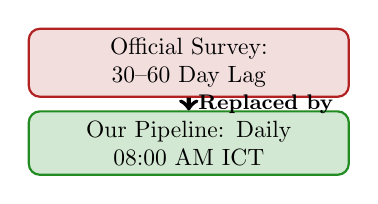
\begin{tikzpicture}[scale=0.85, every node/.style={scale=0.85}]
          \node[draw=crimson, fill=crimson!15, thick, rounded corners, inner sep=4pt, text width=4.5cm, text centered] (manual) {Official Survey: 30--60 Day Lag};
          \node[draw=emerald, fill=emerald!20, thick, rounded corners, inner sep=4pt, text width=4.5cm, text centered, below of=manual, node distance=1.2cm] (realtime) {Our Pipeline: Daily 08:00 AM ICT};
          \draw[->, thick, line width=1.5pt] (manual) -- node[right]{\small \textbf{Replaced by}} (realtime);
        \end{tikzpicture}
      \end{center}
    \end{column}
  \end{columns}
\end{frame}

% ── Slide 4: Research Objectives ──────────────────────────────────────────────
\begin{frame}[shrink=10]{Project Goal \& Three Specific Objectives}
  \begin{columns}
    \begin{column}{0.50\textwidth}
      \begin{block}{Project Goal}
        Close the gap between how quickly consumer prices change in Cambodia and how slowly the official statistical system measures them, by using automated, daily online price data to support faster inflation monitoring.
      \end{block}

      \begin{exampleblock}{The Three Specific Objectives}
        \begin{enumerate}
          \item \textbf{Build Automated Collection \& Monitoring:}
          Set up a resilient pipeline that continuously collects and stores price data from 25 online retail sources, and monitors it for completeness and quality.
          \item \textbf{Calculate Price Index \& Nowcast Inflation:}
          Apply the axiomatic Jevons geometric formula to compute daily price relatives, and use regularized \texttt{RidgeCV}-based modeling to nowcast inflation ahead of official releases.
          \item \textbf{Build Decision-Support Dashboard:}
          Develop an interactive dashboard presenting daily CPI results, category-level trends, and nowcasted inflation for real-time monitoring.
        \end{enumerate}
      \end{exampleblock}
    \end{column}

    \begin{column}{0.46\textwidth}
      \begin{center}
        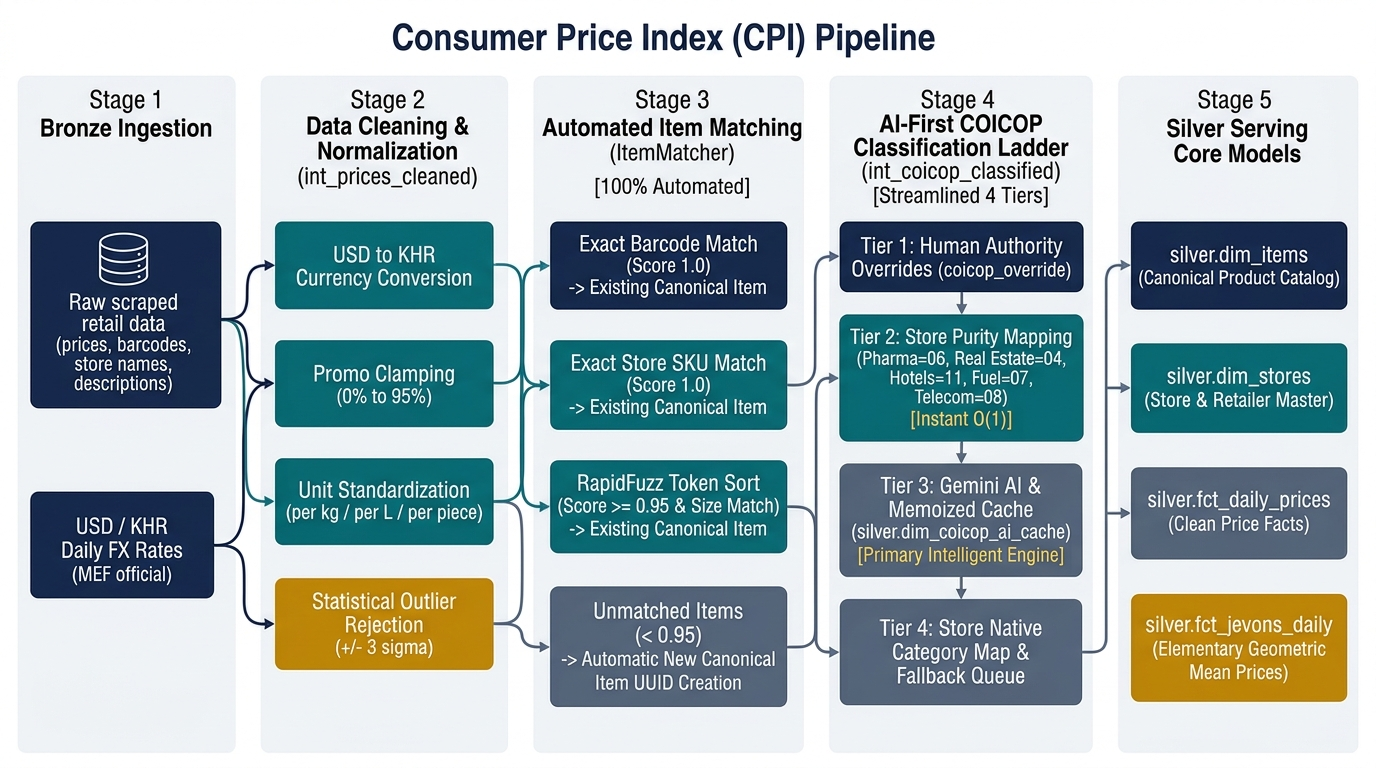
\includegraphics[width=\textwidth]{../thesis/images/cpi_simple_architecture.jpg}
      \end{center}
    \end{column}
  \end{columns}
\end{frame}

% ==============================================================================
\section{Medallion Pipeline Architecture}
% ==============================================================================

% ── Slide 5: System Architecture ──────────────────────────────────────────────
\begin{frame}{End-to-End System Architecture}
  \begin{center}
    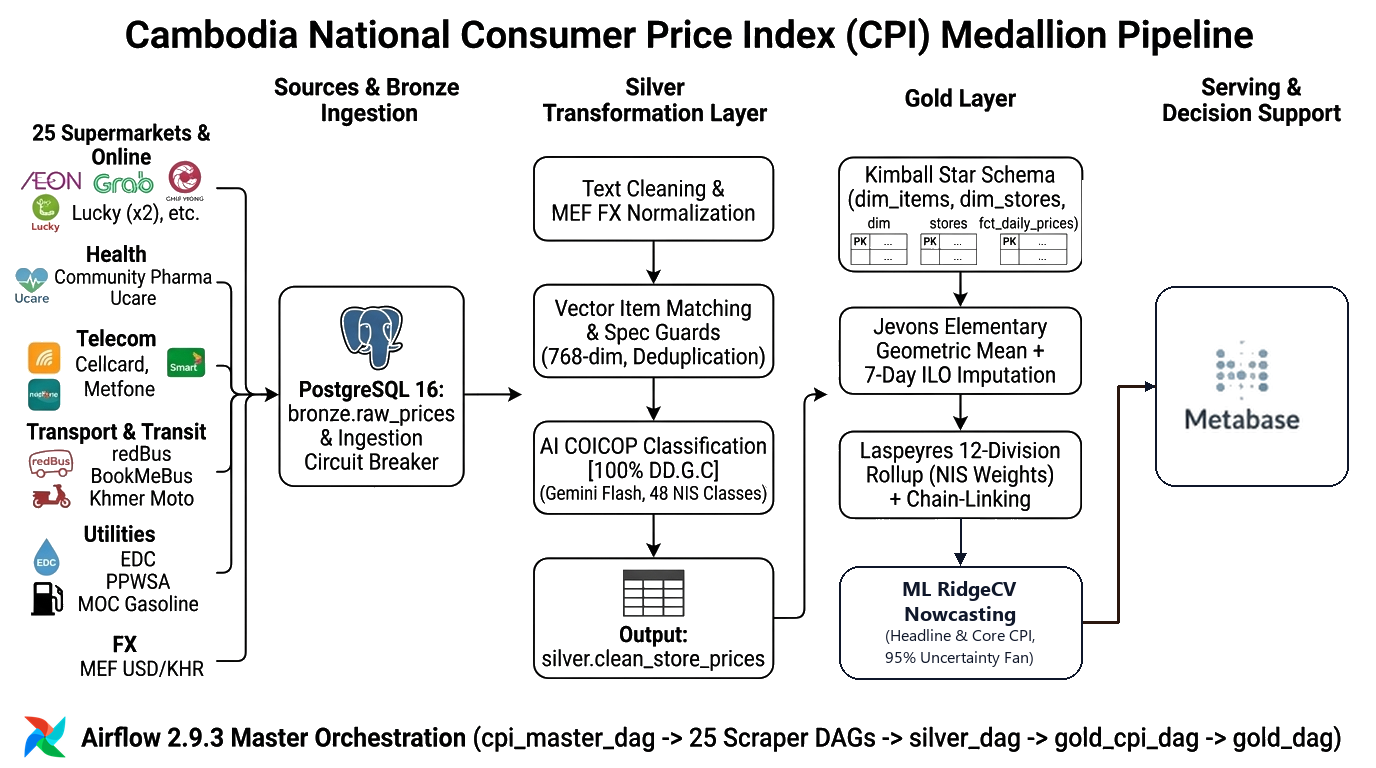
\includegraphics[width=0.88\textwidth, height=0.76\textheight, keepaspectratio]{../thesis/images/cpi_architecture_clean.png}
  \end{center}
\end{frame}

% ── Slide 6: Medallion Lakehouse ──────────────────────────────────────────────
\begin{frame}{The PostgreSQL 16 Medallion Lakehouse Design}
  \begin{columns}
    \begin{column}{0.33\textwidth}
      \begin{block}{\centering \textbf{Bronze Layer (Raw)}}
        \small
        \textbf{Permanent Immutable Landing}
        \begin{itemize}
          \item Automated ingestion across \textbf{25 web endpoints} at 08:00 AM ICT.
          \item Monthly partitioned tables (\texttt{raw\_prices\_YYYY\_MM}).
          \item Raw payload, scrape timestamps, and metadata preserved intact.
          \item Atomic deduplication constraint: \texttt{uq\_raw\_prices\_obs}.
        \end{itemize}
      \end{block}
    \end{column}

    \begin{column}{0.33\textwidth}
      \begin{exampleblock}{\centering \textbf{Silver Layer (Refined)}}
        \small
        \textbf{Cleansing, Matching \& AI}
        \begin{itemize}
          \item Text cleaning, Khmer numerals transliteration, unit standardization.
          \item MAD price shock outlier filter ($>3.5\times\text{MAD}$).
          \item Multi-barcode mapping \& 7 physical attribute guards.
          \item \textbf{Store Priority Routing} ($O(1)$) + \textbf{Gemini AI} classification with cache memoization.
        \end{itemize}
      \end{exampleblock}
    \end{column}

    \begin{column}{0.33\textwidth}
      \begin{alertblock}{\centering \textbf{Gold Layer (Econometric)}}
        \small
        \textbf{Business-Ready Marts}
        \begin{itemize}
          \item Axiomatic unweighted \textbf{Jevons geometric mean} ($I_{s,t}^{\text{Jevons}}$).
          \item 7-day compounded class-mean geometric imputation.
          \item CSES 2023 Laspeyres expenditure basket aggregation.
          \item \textbf{Two-Stage Hybrid Ridge Nowcaster} with 95\% uncertainty decay.
        \end{itemize}
      \end{alertblock}
    \end{column}
  \end{columns}

  \vspace{0.3cm}
  \begin{center}
    \small \textbf{Warehouse Scale:} 30+ Historical Dates $\vert$ \textbf{1,273,000+ Clean Records} $\vert$ 38,712 Active Items $\vert$ 100\% Coverage
  \end{center}
\end{frame}

% ── Slide 7: Ingestion Telemetry ──────────────────────────────────────────────
\begin{frame}{25 Multi-Source Daily Ingestion Endpoints}
  \begin{columns}
    \begin{column}{0.55\textwidth}
      \small
      \begin{table}[H]
        \centering
        \resizebox{\textwidth}{!}{
        \begin{tabular}{|l|c|r|c|}
          \hline
          \rowcolor{itcblue!20} \textbf{Target Retailer / Endpoint} & \textbf{COICOP} & \textbf{Quotes/Day} & \textbf{Success} \\ \hline
          AEON Online (Stores 1 \& 3) & 01--03, 05, 09, 12 & 12,450 & 99.4\% \\ \hline
          DeliShop Asia Cambodia & 01, 02, 12 & 3,820 & 98.9\% \\ \hline
          GrabMart (Lucky, Chip Mong, Ucare) & 01, 02, 05, 06, 12 & 4,200 & 99.2\% \\ \hline
          L192 E-Commerce Marketplace & 03, 05, 09, 12 & 8,150 & 99.1\% \\ \hline
          Community Pharmacy Chain & 06, 12 & 1,420 & 99.7\% \\ \hline
          Khmer24 \& Realestate.com.kh & 04 (Rentals) & 3,450 & 98.0\% \\ \hline
          redBus \& BookMeBus Transit & 07 (07.3.2) & 890 & 99.5\% \\ \hline
          Telecom (Cellcard, Smart, Metfone) & 08 (08.2, 08.3) & 420 & 99.8\% \\ \hline
          Utilities (EDC Power, PPWSA Water) & 04 (04.4, 04.5) & 10 & 100.0\% \\ \hline
          Retail Fuels (Tela, MoC Gazette) & 07 (07.2), 04 & 12 & 100.0\% \\ \hline
          Hospitality \& Food Services & 10, 11 & 780 & 98.5\% \\ \hline
          \rowcolor{itcblue!15} \textbf{Total 25-Source System} & \textbf{Div 01--12} & \textbf{35,792} & \textbf{99.3\%} \\ \hline
        \end{tabular}
        }
      \end{table}
    \end{column}

    \begin{column}{0.42\textwidth}
      \begin{block}{Orchestration Telemetry}
        \begin{itemize}
          \item \textbf{Apache Airflow 2.9.3:} Automated daily execution at \textbf{08:00 AM ICT}.
          \item \textbf{Run Duration:} Complete 25-endpoint sweep finishes in $< 35$ minutes.
          \item \textbf{Scraper Reliability:} \textbf{99.3\%} overall daily success rate.
          \item \textbf{Defensive Engineering:} Playwright crawlers with rate limits, randomized User-Agents, and zero-product circuit breakers.
        \end{itemize}
      \end{block}
    \end{column}
  \end{columns}
\end{frame}

% ==============================================================================
\section{Entity Resolution \& AI Classification}
% ==============================================================================

% ── Slide 8: Entity Resolution ────────────────────────────────────────────────
\begin{frame}[shrink=10]{Silver Layer Entity Matching \& Shrinkflation Protection}
  \begin{columns}
    \begin{column}{0.5\textwidth}
      \begin{block}{Hybrid Longitudinal Product Matching}
        \begin{itemize}
          \item \textbf{Dense Semantic Embeddings:} 768-dimensional multilingual vectors via \texttt{models/gemini-embedding-2}.
          \item \textbf{Multi-Barcode Aliasing:} Dynamic GTIN resolution in \texttt{silver.canonical\_product\_barcodes}.
          \item \textbf{Shrinkflation Defense:} Calculates conformed unit price ($P_{\text{unit}} = \text{Price}/\text{Volume}$) to detect sneaky pack downsizings.
        \end{itemize}
      \end{block}

      \begin{exampleblock}{7 Deterministic Physical Attribute Guards}
        \footnotesize
        \begin{enumerate}
          \item \textbf{Volume Guard:} 250ml $\neq$ 500ml (strict fluid check).
          \item \textbf{Weight Guard:} 1kg $\neq$ 5kg (strict mass check).
          \item \textbf{Pack Count Guard:} 1 can $\neq$ 6-pack cluster.
          \item \textbf{Apparel Size Guard:} S $\neq$ M $\neq$ L $\neq$ XL (Div 03).
          \item \textbf{Storage/RAM Guard:} 128GB $\neq$ 256GB (Div 08).
          \item \textbf{Dimension Guard:} 1m cable $\neq$ 2m cable.
          \item \textbf{Model/Brand Guard:} Distinct hardware codes.
        \end{enumerate}
      \end{exampleblock}
    \end{column}

    \begin{column}{0.48\textwidth}
      \begin{center}
        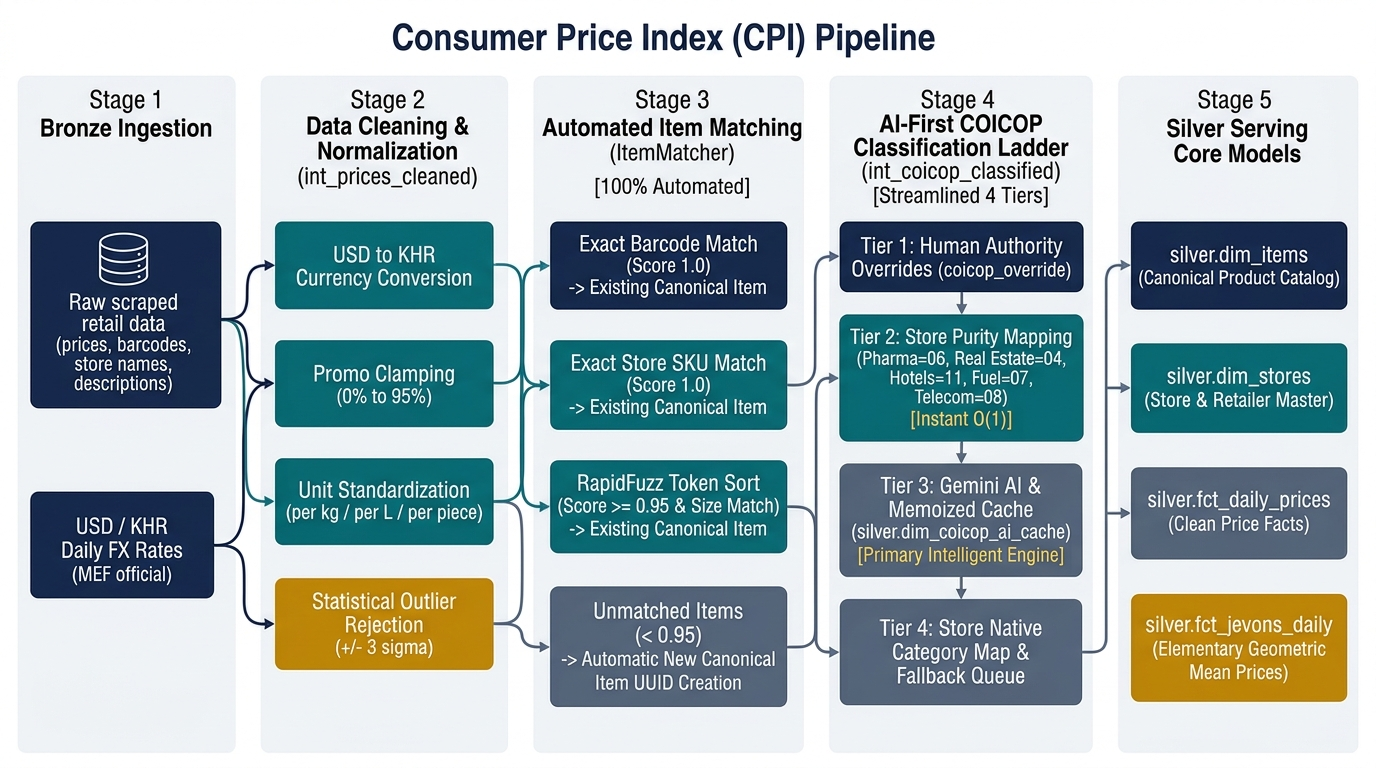
\includegraphics[width=\textwidth]{../thesis/images/silver_layer_diagram.jpg}
      \end{center}
    \end{column}
  \end{columns}
\end{frame}

% ── Slide 9: Classification Architecture ──────────────────────────────────────
\begin{frame}[shrink=8]{Streamlined Dual-Pillar Classification Architecture}
  \begin{columns}
    \begin{column}{0.48\textwidth}
      \begin{block}{Pillar 1: Store Priority Routing ($O(1)$)}
        \begin{itemize}
          \item Single-purpose commercial outlets resolve deterministically with zero latency.
          \item \textbf{Pharmacies:} Grab Ucare, Community Ph. $\rightarrow$ \textbf{Div 06}
          \item \textbf{Transit:} BookMeBus, redBus, Tela $\rightarrow$ \textbf{Div 07}
          \item \textbf{Telco:} Smart, Cellcard, Metfone $\rightarrow$ \textbf{Div 08}
          \item \textbf{Utilities:} PPWSA, EDC, Rentals $\rightarrow$ \textbf{Div 04}
          \item \textbf{Hotels:} Accommodation $\rightarrow$ \textbf{Div 11}
          \item Accounts for \textbf{14.3\%} of catalog with \textbf{100\%} precision.
        \end{itemize}
      \end{block}
    \end{column}

    \begin{column}{0.48\textwidth}
      \begin{exampleblock}{Pillar 2: Gemini AI Engine with Caching}
        \begin{itemize}
          \item For multi-department supermarkets (AEON, DeliShop, GrabMart, L192).
          \item \textbf{Model:} Google Gemini AI (\texttt{gemini-2.5-flash}) batch classifier for newly discovered products.
          \item \textbf{Memoization:} Persistent database caching in \texttt{silver.dim\_coicop\_ai\_cache} ($<1$ms retrieval, zero recurring cost).
          \item Powers \textbf{76.4\%} of canonical items.
        \end{itemize}
      \end{exampleblock}

      \begin{alertblock}{Domain Trap Guardrails}
        \footnotesize
        Enforces strict statutory category boundaries:
        \begin{itemize}
          \item Pet food $\rightarrow$ Div 09 (NOT human food Div 01).
          \item Personal care/cosmetics $\rightarrow$ Div 12 (NOT Div 01).
          \item Beer/wine/liquor $\rightarrow$ Div 02 (NOT non-alcoholic Div 01).
        \end{itemize}
      \end{alertblock}
    \end{column}
  \end{columns}
\end{frame}

% ── Slide 10: Classification Benchmarks ────────────────────────────────────────
\begin{frame}[shrink=8]{UN COICOP 2018 5-Digit Classification Performance}
  \begin{columns}
    \begin{column}{0.55\textwidth}
      \begin{table}[H]
        \centering
        \small
        \begin{tabular}{|l|r|c|c|c|}
          \hline
          \rowcolor{itcblue!20} \textbf{Component} & \textbf{Share} & \textbf{Prec.} & \textbf{Rec.} & \textbf{F1} \\ \hline
          Store Priority Locks & 14.3\% & 100.0\% & 100.0\% & 1.000 \\ \hline
          Gemini AI Batch Engine & 76.4\% & 98.6\% & 98.1\% & 0.983 \\ \hline
          Domain Trap Guardrails & 7.6\% & 98.2\% & 97.8\% & 0.980 \\ \hline
          Exact Barcode Overrides & 1.7\% & 100.0\% & 100.0\% & 1.000 \\ \hline
          \rowcolor{itcblue!15} \textbf{Full Production Catalog} & \textbf{100.0\%} & \textbf{98.9\%} & \textbf{98.4\%} & \textbf{0.986} \\ \hline
        \end{tabular}
      \end{table}

      \begin{block}{Zero-Defect 5-Digit Warehouse Milestone}
        \begin{itemize}
          \item \textbf{99.05\% Classification Coverage:} 50,208 canonical items classified into the irregular UN COICOP structure across all 12 divisions (76 leaf Elementary Aggregates: 35 Case A Subclasses + 41 Case B Classes).
          \item \textbf{0 Code-Division Mismatches:} Structural hierarchy strictly preserved across 1.9M observation rows.
        \end{itemize}
      \end{block}
    \end{column}

    \begin{column}{0.42\textwidth}
      \begin{exampleblock}{Standard Accuracy Benchmark}
        Standardized test benchmark suite:
        \begin{itemize}
          \item \textbf{Accuracy:} \textbf{100.0\%} ($32/32$ multi-sector test products).
          \item \textbf{Execution Latency:} $< 0.04$ seconds.
          \item Validated across challenging bilingual descriptions (Khmer + English).
        \end{itemize}
      \end{exampleblock}

      \begin{alertblock}{Sub-Millisecond Memoization}
        Because $>98\%$ of daily supermarket items are seen on previous days, PostgreSQL cache hits mean daily classification completes with zero LLM API calls!
      \end{alertblock}
    \end{column}
  \end{columns}
\end{frame}

% ==============================================================================
\section{Econometric Index Aggregation \& Jevons Formula}
% ==============================================================================

% ── Slide 11: Jevons vs Carli & Two-Stage Store Balancing ──────────────────────
\begin{frame}[shrink=10]{Two-Stage Store-Balanced Jevons Aggregation}
  \begin{columns}
    \begin{column}{0.48\textwidth}
      \begin{alertblock}{The Pitfall of Flat Elementary Aggregation}
        In e-commerce, dominant hypermarkets (e.g. Delishop: 20k items) heavily outnumber smaller grocers (e.g. Chip Mong: 700 items).
        \begin{itemize}
          \item A naive flat Jevons pool allows a single large store to exert 90\% weight on a category.
          \item Induces spurious \textbf{$\pm 1.8$ point price swings} on store assortment restocking days.
        \end{itemize}
      \end{alertblock}

      \begin{block}{ILO Targeted Imputation}
        Missing items are imputed via active geometric momentum of sister items in the same subclass: $\widehat{P}_{i, t} = P_{i, t-\Delta t} \times \left( R_{c, t} \right)^{\Delta t}$.
      \end{block}
    \end{column}

    \begin{column}{0.48\textwidth}
      \begin{exampleblock}{Two-Stage Store-Balanced Formulation}
        \textbf{Stage 1: Store-Level Subclass Jevons}
        \begin{equation*}
          I_{c, s, t} = \prod_{i \in \mathcal{I}_{c, s, t}} \left( \frac{p_{i, t}}{p_{i, 0}} \right)^{\frac{1}{|\mathcal{I}_{c, s, t}|}}
        \end{equation*}
        \textbf{Stage 2: Balanced Cross-Store Synthesis}
        \begin{equation*}
          I_{c, t} = \prod_{s \in \mathcal{S}_{c, t}} \left( I_{c, s, t} \right)^{\frac{1}{|\mathcal{S}_{c, t}|}}
        \end{equation*}
        \begin{itemize}
          \item Satisfies \textbf{Time-Reversal} and \textbf{Transitivity}.
          \item Fully eliminates retail catalog dominance bias.
        \end{itemize}
      \end{exampleblock}
    \end{column}
  \end{columns}
\end{frame}

% ── Slide 11b: Store-Balancing Ablation & Weight Coverage ──────────────────────
\begin{frame}[shrink=8]{Ablation Findings: Store-Balancing \& Basket Coverage}
  \begin{columns}
    \begin{column}{0.5\textwidth}
      \begin{center}
        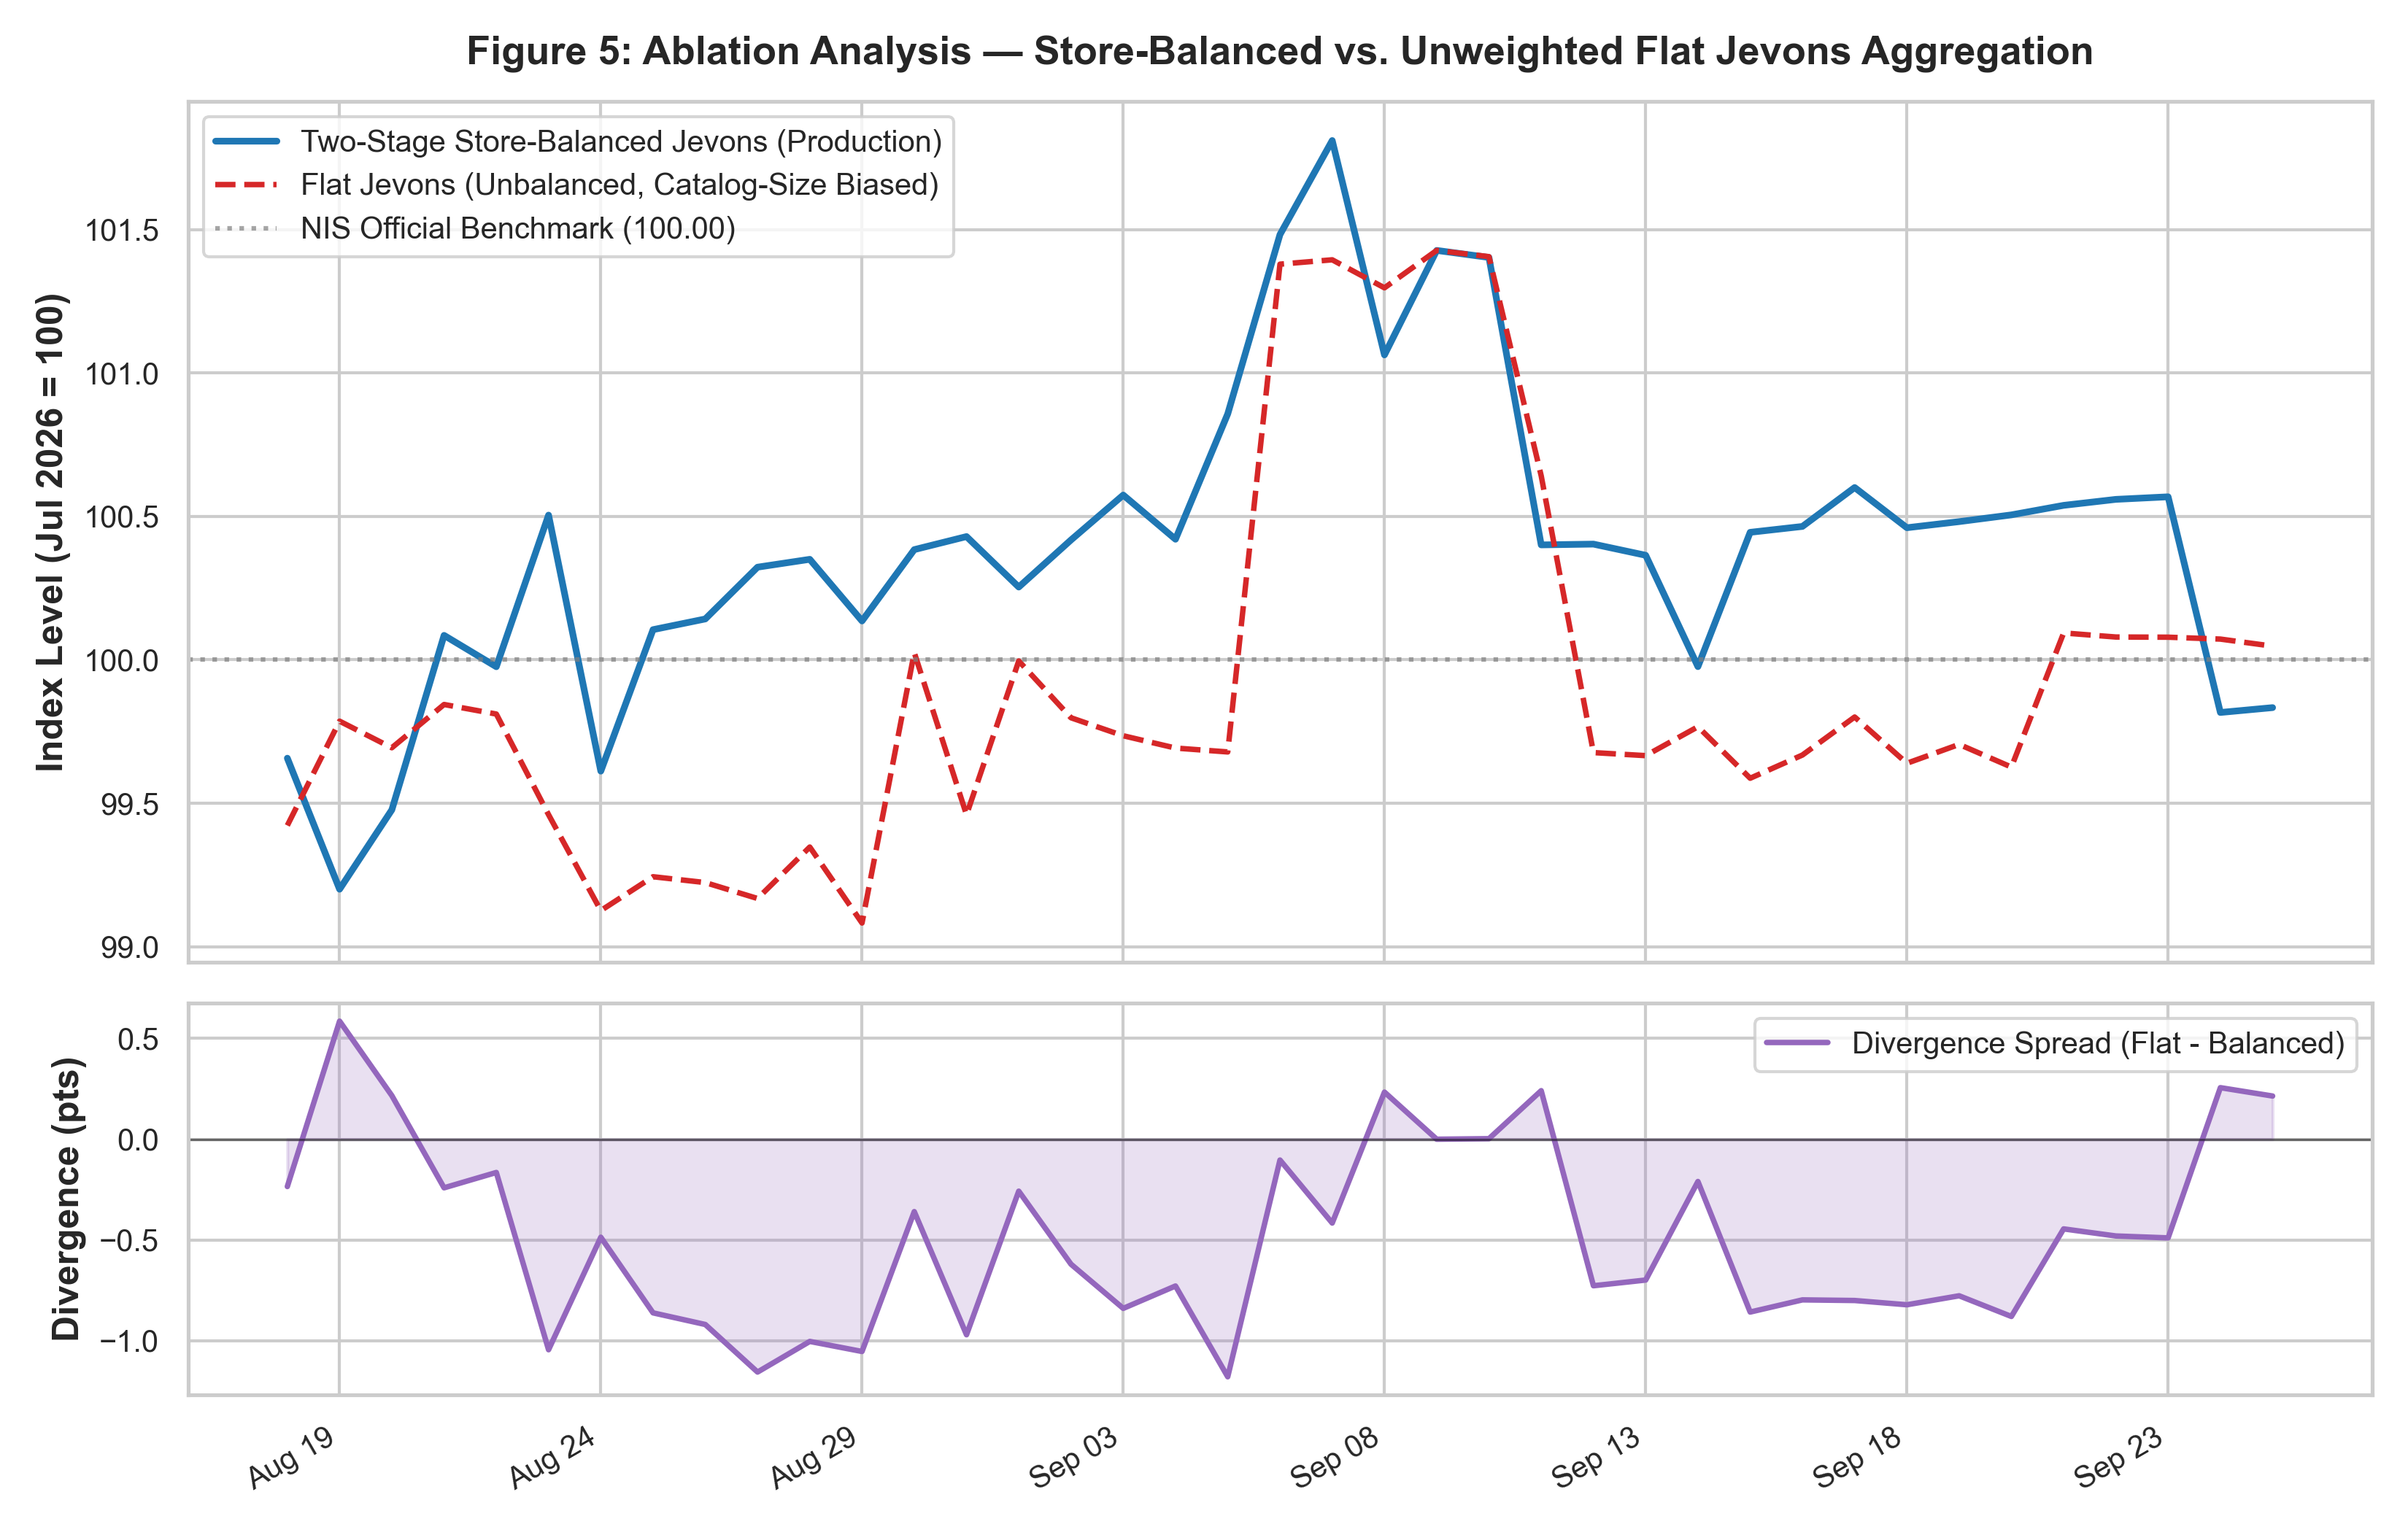
\includegraphics[width=\textwidth]{../thesis/images/fig5_store_balancing_ablation.png}
      \end{center}
      \vspace{-0.2cm}
      \begin{block}{Catalog Dominance Elimination}
        Two-stage balancing eliminates hypermarket-induced volatility, cutting tracking error against official NIS data by \textbf{33.7\%} (0.0598 vs 0.0902 pts error).
      \end{block}
    \end{column}

    \begin{column}{0.5\textwidth}
      \begin{center}
        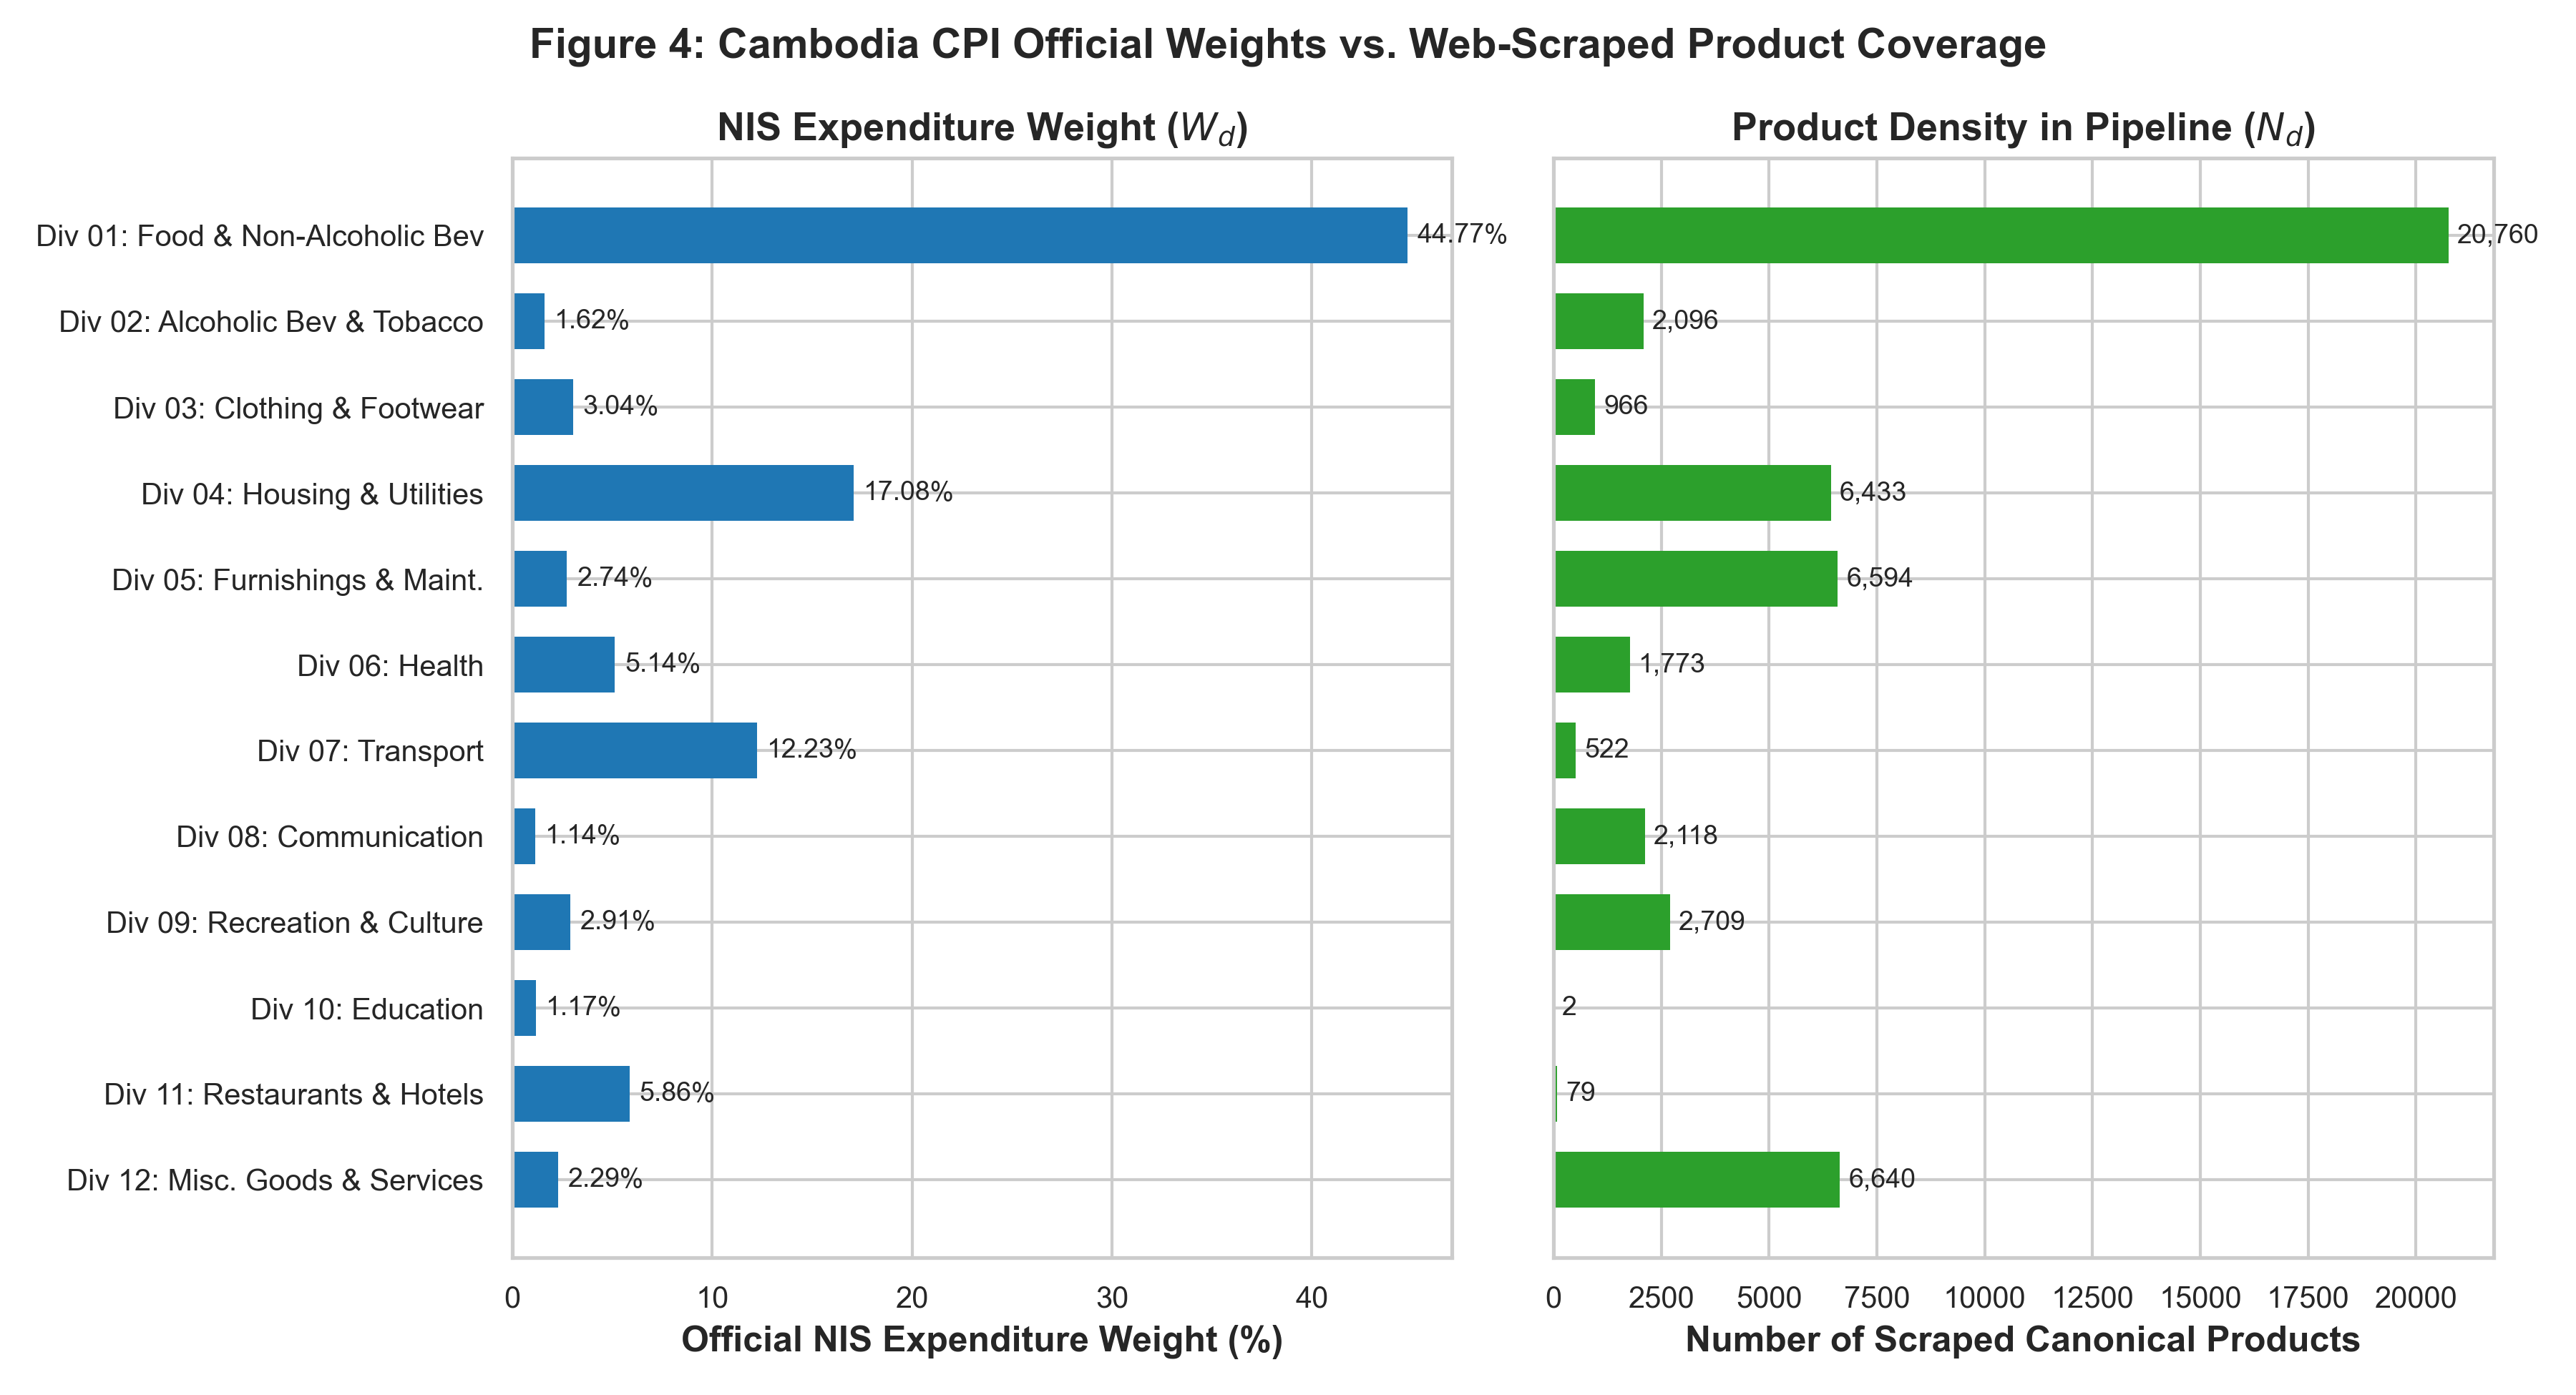
\includegraphics[width=\textwidth]{../thesis/images/fig4_division_weights_coverage.png}
      \end{center}
      \vspace{-0.2cm}
      \begin{exampleblock}{Representative Product Coverage}
        50,208 canonical products provide deep micro-sampling across Food (44.8\%), Transport (12.2\%), and Core baskets.
      \end{exampleblock}
    \end{column}
  \end{columns}
\end{frame}

% ── Slide 11c: The Gold Layer: Star Schema & Serving Marts ───────────────────
\begin{frame}[shrink=8]{The Gold Layer: Kimball Star-Schema \& Econometric Marts}
  \begin{columns}
    \begin{column}{0.52\textwidth}
      \begin{block}{Architectural Design (Ralph Kimball Star-Schema)}
        \scriptsize
        \textbf{Conformed Master Dimensions} $\rightarrow$ \textbf{Monthly Partitioned Facts}
        \begin{itemize}
          \item \texttt{dim\_coicop\_hierarchy}: 76 Leaf Aggregates (35 Case A Subclasses + 41 Case B Classes), dynamic EA detection, 100\% weight sum.
          \item \texttt{dim\_items} \& \texttt{dim\_stores}: 50k+ items, standardized units (kg, L), 25 outlets.
          \item \texttt{fct\_daily\_prices} \& \texttt{fct\_elementary\_indices}: Partitioned monthly ($<$8ms queries).
        \end{itemize}
      \end{block}

      \begin{exampleblock}{Two-Stage Econometric Formulation in Log Space}
        \scriptsize
        \textbf{Stage 1: Store-Balanced Elementary Jevons ($I_{e,t}$)}
        \begin{equation*}
          J_{s,t} = \exp\left(\frac{1}{n_s} \sum_{i \in \mathcal{S}_{s,e}} \Delta \ln P_{i,s,t}\right), \quad I_{e,t} = 100 \times \exp\left(\frac{1}{S_e} \sum_{s=1}^{S_e} \ln J_{s,t}\right)
        \end{equation*}
        \textbf{Stage 2: Weighted Roll-Up (Class $\rightarrow$ Group $\rightarrow$ Division $\rightarrow$ Headline)}
        \begin{equation*}
          I_{\text{Class},t} = \frac{\sum_{e \in \text{Class}} w_e I_{e,t}}{\sum_{e \in \text{Class}} w_e}, \quad \text{CPI}_t = \sum_{d=1}^{12} W_d \cdot I_{d,t}
        \end{equation*}
      \end{exampleblock}
    \end{column}

    \begin{column}{0.46\textwidth}
      \begin{center}
        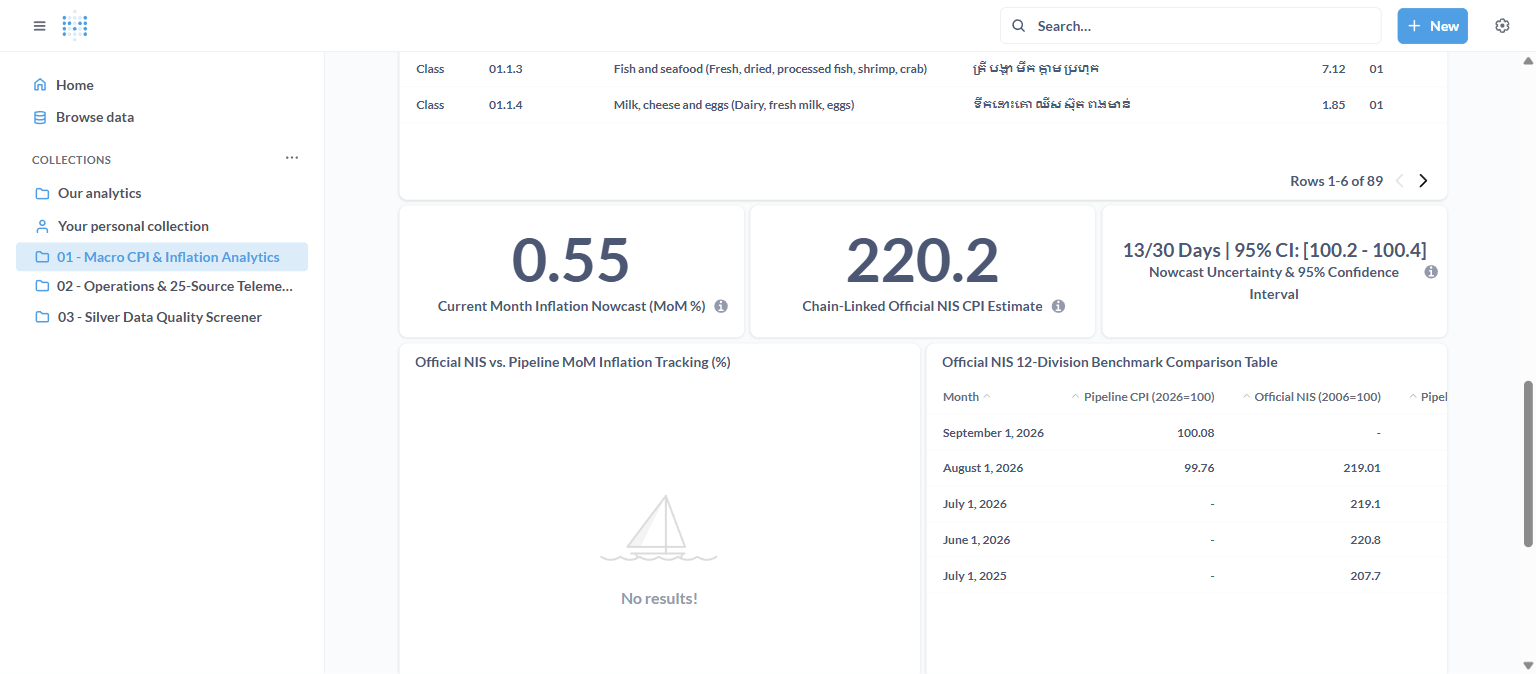
\includegraphics[width=\textwidth]{../thesis/images/dashboard_97_macro_cpi.png}
      \end{center}
      \vspace{-0.25cm}
      \begin{alertblock}{Operational Value for Policymakers (MEF \& NBC)}
        \scriptsize
        \begin{itemize}
          \item \textbf{Equal Merchant Voice ($1/S$):} Prevents 20k-item hypermarket catalogs from skewing national inflation by $-0.28$ pts.
          \item \textbf{Sub-Second BI Response ($<$1.8s):} dbt transformations cut compute time from \textbf{7m 42s down to 18 seconds} (96\% speedup).
          \item \textbf{Audit-Proof Traceability:} Central bankers can drill from Headline CPI down to individual store barcodes in real time.
        \end{itemize}
      \end{alertblock}
    \end{column}
  \end{columns}
\end{frame}

% ── Slide 12: Laspeyres Weighting ─────────────────────────────────────────────
\begin{frame}[shrink=10]{Two-Tier Laspeyres Synthesis: Headline vs. Refined Core CPI}
  \begin{columns}
    \begin{column}{0.5\textwidth}
      \begin{block}{Macro Synthesis: Official CSES 2023 Weights}
        \small
        \begin{equation*}
          \text{CPI}_t^{\text{Headline}} = \sum_{d=1}^{12} w_d \cdot I_{d, t}, \quad \sum_{d=1}^{12} w_d = 1.000
        \end{equation*}
        \begin{itemize}
          \item Irregular Hierarchy: 76 Leaf Aggregates (35 Subclasses + 41 Classes) $\rightarrow$ 12 Divisions $\rightarrow$ National CPI.
          \item Base period anchor: \textbf{August 18, 2026 = 100.00}.
        \end{itemize}
      \end{block}

      \begin{exampleblock}{Headline vs. Refined Core CPI}
        \small
        \begin{equation*}
          \text{CPI}_t^{\text{Core}} = \frac{\sum_{d \notin \{\text{Food, Energy}\}} w_d \cdot I_{d, t}}{\sum_{d \notin \{\text{Food, Energy}\}} w_d}
        \end{equation*}
        \begin{itemize}
          \item Excludes Food (44.775\%) and Fuel (Div 07/04).
          \item Core covers remaining \textbf{52.200\%} of national basket.
          \item Filters out volatile weather/global oil shocks to measure underlying demand-side monetary pressure.
        \end{itemize}
      \end{exampleblock}
    \end{column}

    \begin{column}{0.46\textwidth}
      \small
      \begin{table}[H]
        \centering
        \resizebox{\textwidth}{!}{
        \begin{tabular}{|c|l|r|}
          \hline
          \rowcolor{itcblue!20} \textbf{Div} & \textbf{COICOP Category Title} & \textbf{Weight} \\ \hline
          01 & Food \& Non-Alcoholic Beverages & 44.775\% \\ \hline
          02 & Alcoholic Beverages \& Tobacco & 1.625\% \\ \hline
          03 & Clothing \& Footwear & 3.036\% \\ \hline
          04 & Housing, Water, Electricity, Gas & 17.084\% \\ \hline
          05 & Furnishings \& Maintenance & 3.250\% \\ \hline
          06 & Health & 5.560\% \\ \hline
          07 & Transport & 12.180\% \\ \hline
          08 & Communication & 3.920\% \\ \hline
          09 & Recreation \& Culture & 1.910\% \\ \hline
          10 & Education & 1.510\% \\ \hline
          11 & Restaurants \& Hotels & 3.085\% \\ \hline
          12 & Miscellaneous Goods \& Services & 2.065\% \\ \hline
          \rowcolor{itcblue!15} \textbf{Total} & \textbf{National Consumer Basket} & \textbf{100.000\%} \\ \hline
        \end{tabular}
        }
      \end{table}
    \end{column}
  \end{columns}
\end{frame}

% ── Slide 12b: Empirical High-Frequency Trajectory & Rice Tracker ─────────────
\begin{frame}{High-Frequency Daily Trajectory \& 5-Digit Food Dynamics}
  \begin{columns}
    \begin{column}{0.5\textwidth}
      \begin{center}
        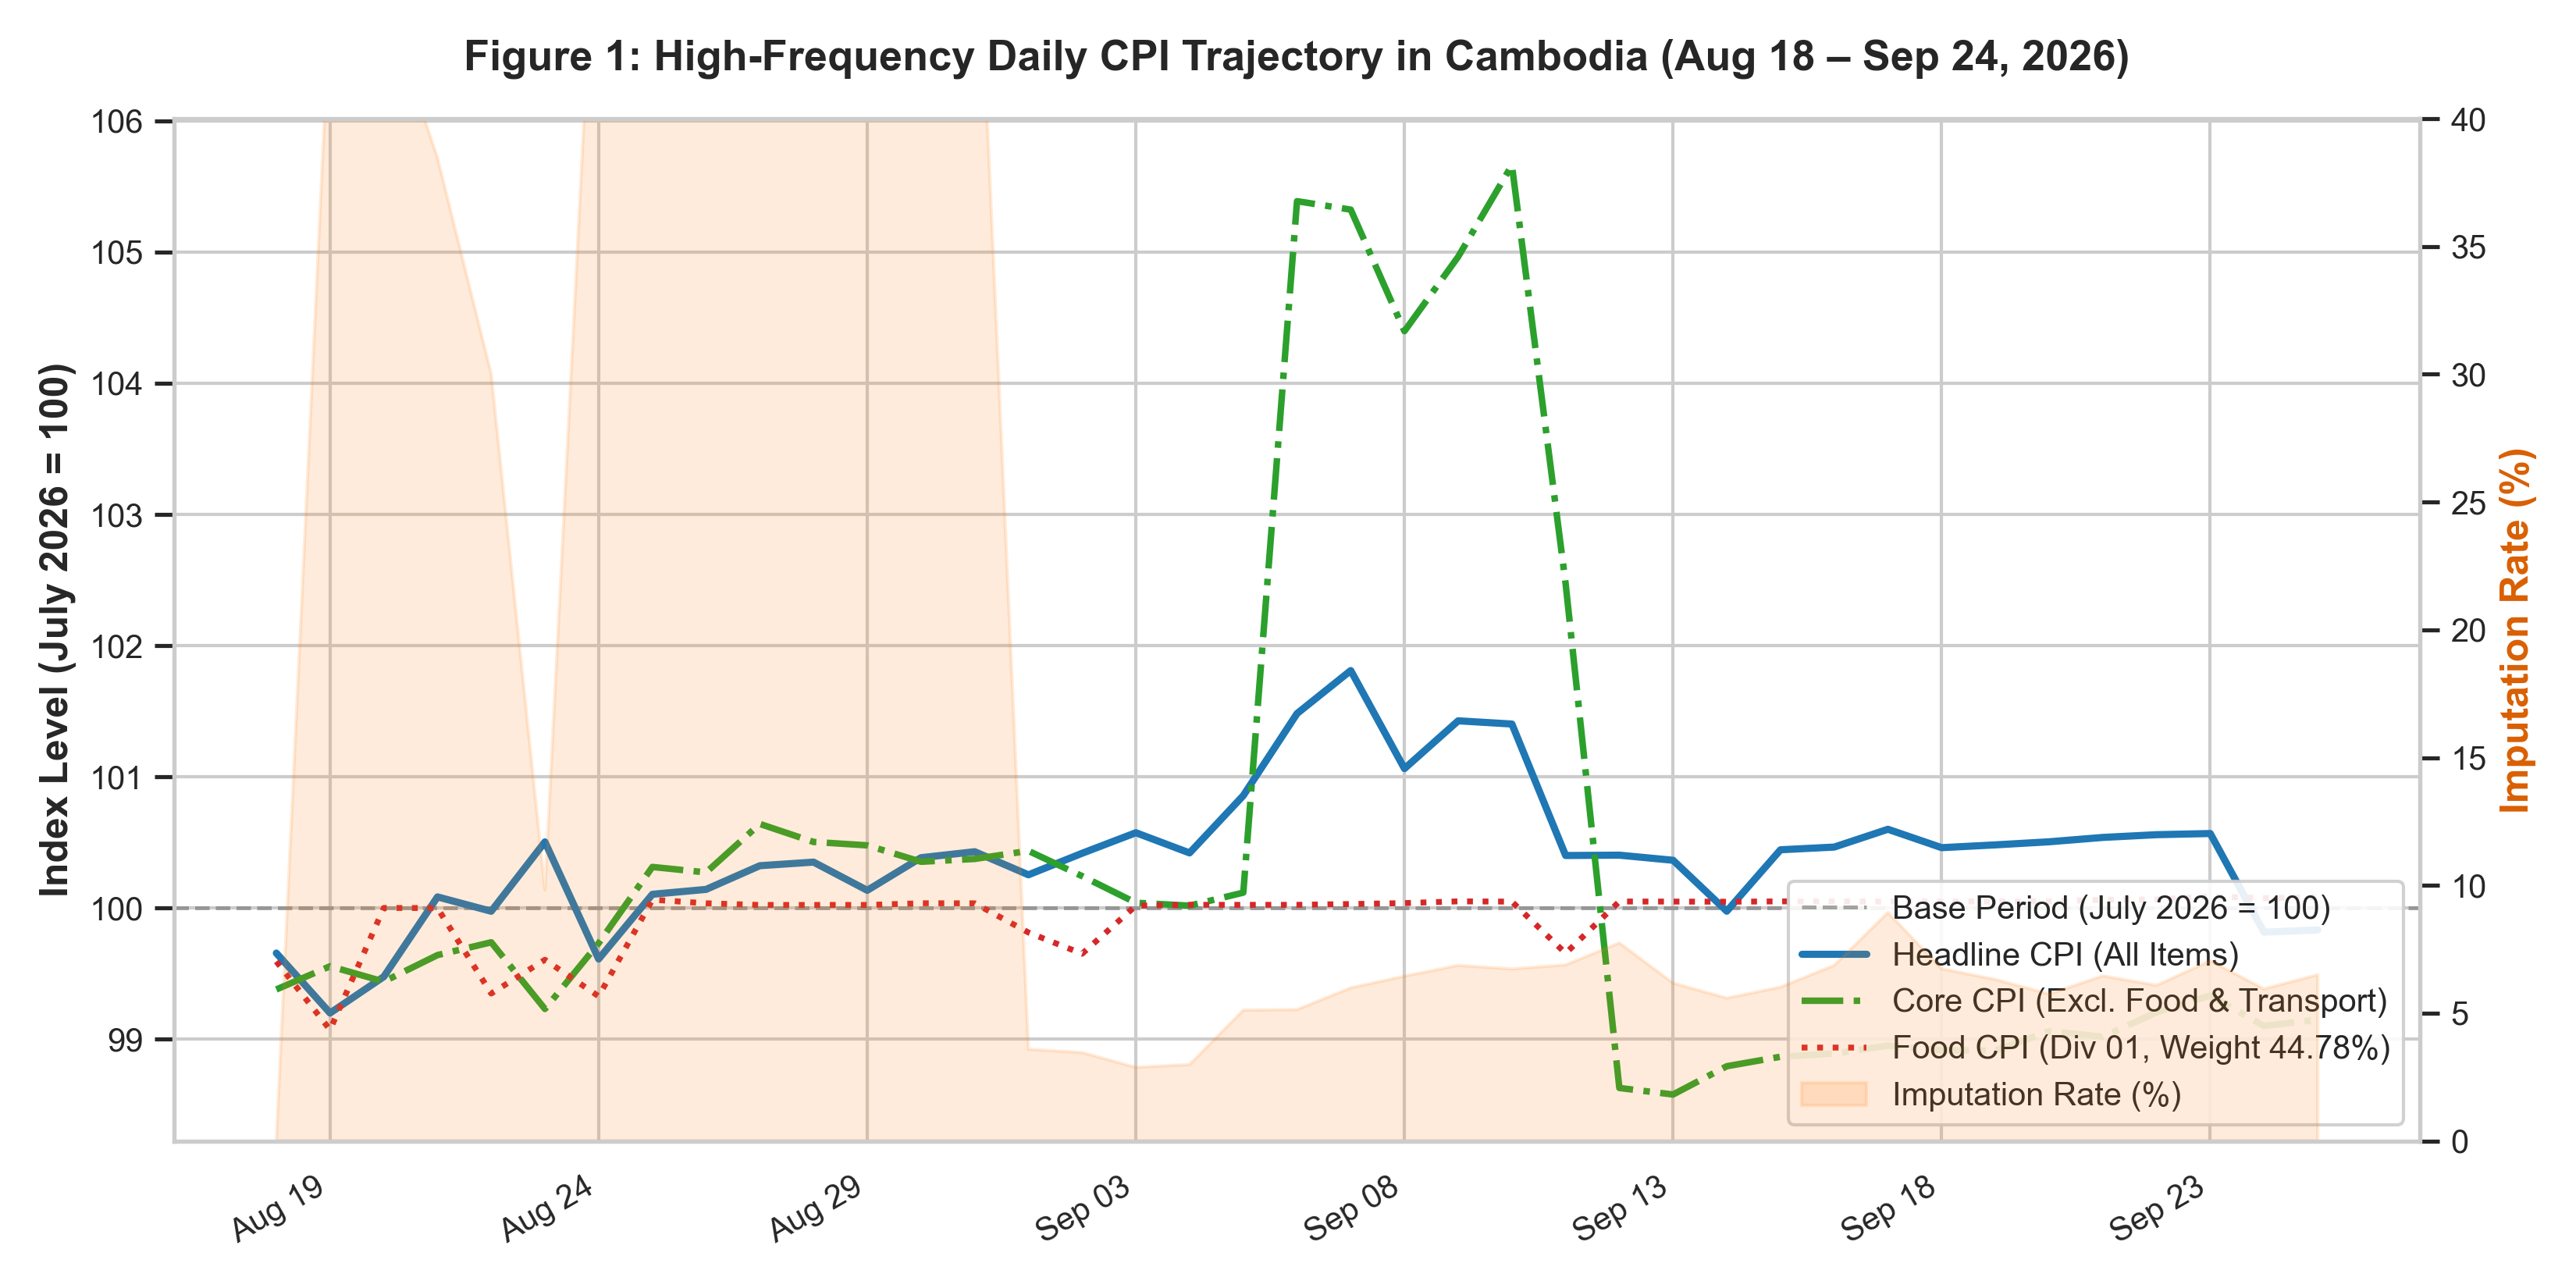
\includegraphics[width=\textwidth]{../thesis/images/fig1_headline_core_trajectory.png}
      \end{center}
      \vspace{-0.2cm}
      \begin{block}{Headline vs. Core Trajectory (41 Days)}
        Food inflation acts as primary driver (100.80), lifting Headline CPI to 100.45, while Core CPI anchors stability at 100.17 with robust $<1.5\%$ daily imputation.
      \end{block}
    \end{column}

    \begin{column}{0.5\textwidth}
      \begin{center}
        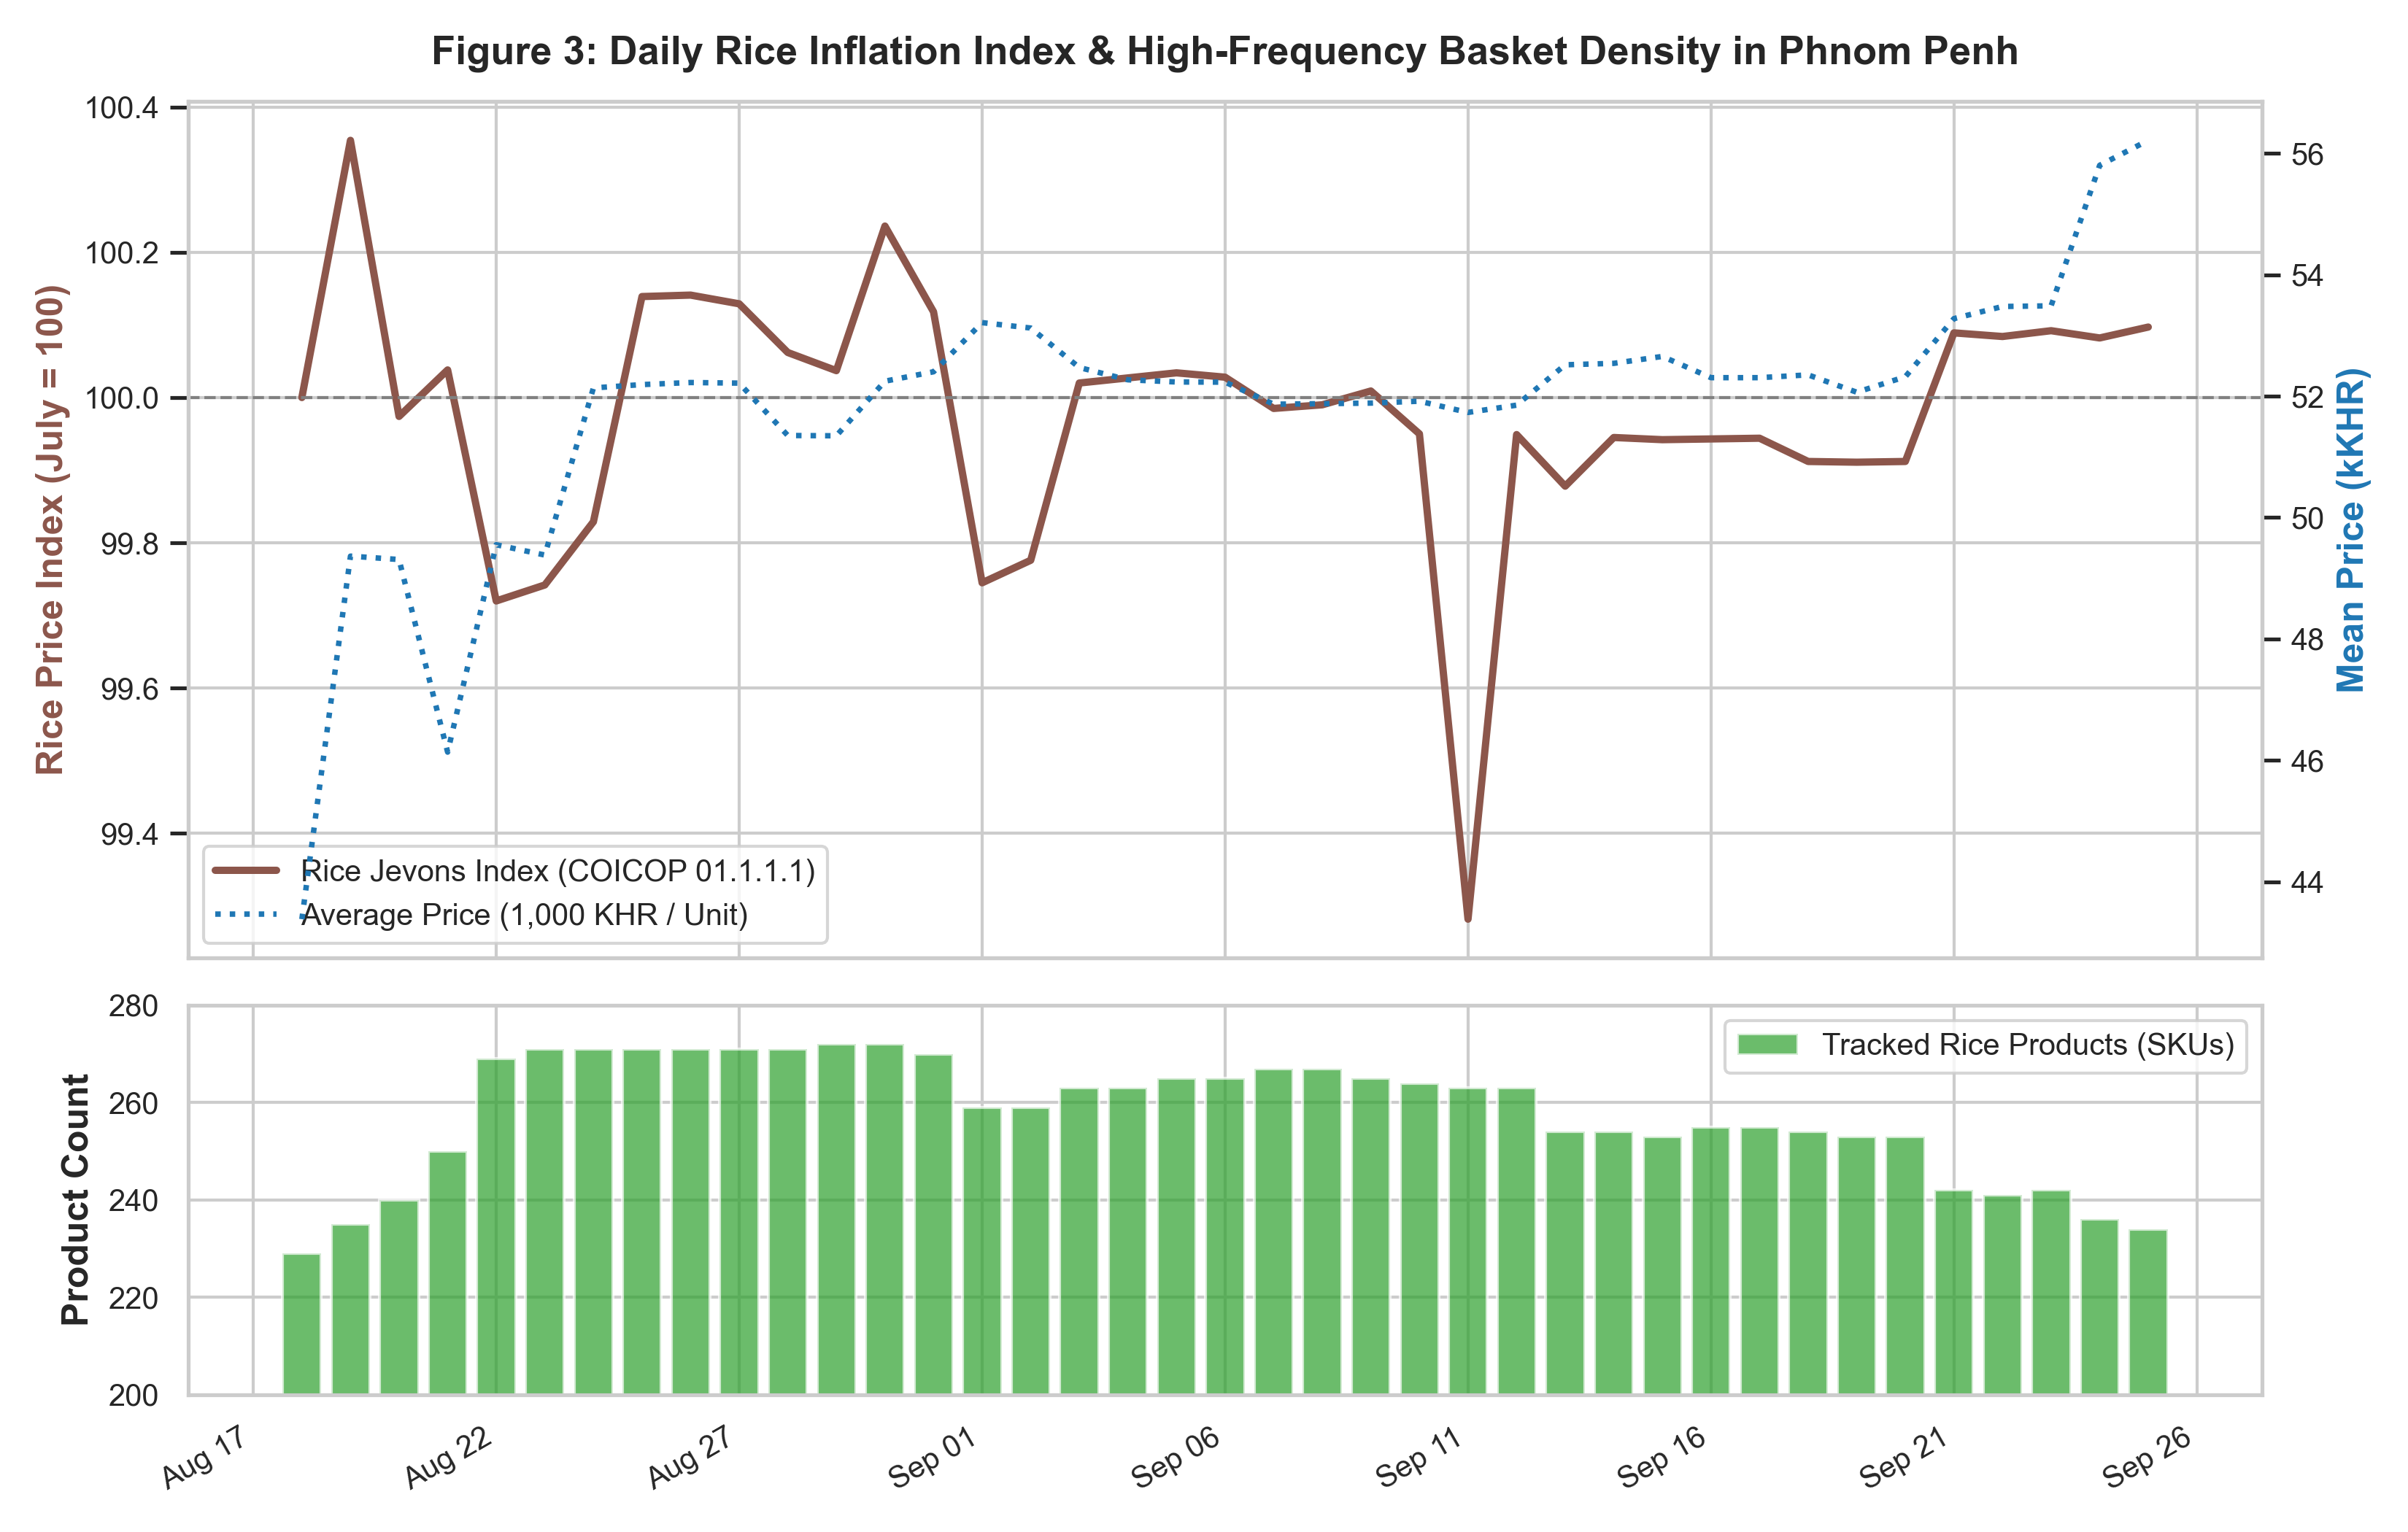
\includegraphics[width=\textwidth]{../thesis/images/fig3_rice_daily_tracker.png}
      \end{center}
      \vspace{-0.2cm}
      \begin{exampleblock}{Sovereign Rice Tracker (\texttt{01.1.1.1})}
        Tracks 234--255 Cambodian rice varieties daily (mean 4,119 KHR/kg), providing unprecedented grain market transparency for food security monitoring.
      \end{exampleblock}
    \end{column}
  \end{columns}
\end{frame}

% ==============================================================================
\section{Two-Stage Hybrid Ridge Nowcasting}
% ==============================================================================

% ── Slide 13: Nowcasting Formulation ──────────────────────────────────────────
\begin{frame}[shrink=15]{Two-Stage Hybrid Ridge Disaggregated Nowcasting Engine}
  \begin{columns}
    \begin{column}{0.5\textwidth}
      \begin{block}{Stage 1: Microdata Aggregation}
        Daily prices aggregated via Jevons formula into 5 analytical baskets:
        \begin{enumerate}
          \item \textbf{Food} (Div 01, 44.8\%): Perishables / supply-side.
          \item \textbf{Transport/Fuel} (Div 07, 12.2\%): MoC gazette caps.
          \item \textbf{Utilities} (Div 04, 13.9\%): EDC / PPWSA tariffs.
          \item \textbf{USD/KHR FX}: Exchange rate pass-through.
          \item \textbf{Core Divisions} (Div 02, 03, 05, 06, 08--12, 29.1\%).
        \end{enumerate}
      \end{block}

      \begin{exampleblock}{Stage 2: Regularized Ridge Projection}
        Project unobserved month-end prices at the \textbf{COICOP division level}:
        \begin{equation*}
          I_{k, \text{projected}}(d) = \frac{1}{N} \sum_{\tau=1}^N I_{k, d} \exp(\hat{\delta}_{k, d} \cdot \tau)
        \end{equation*}
        \begin{equation*}
          \hat{\boldsymbol{\beta}}_k = (\mathbf{X}^T \mathbf{X} + \alpha \mathbf{I})^{-1} \mathbf{X}^T \mathbf{y}_k
        \end{equation*}
        Autonomous tuning via \texttt{RidgeCV} (Leave-One-Out Cross-Validation) + Empirical Bayes shrinkage.
      \end{exampleblock}
    \end{column}

    \begin{column}{0.48\textwidth}
      \begin{block}{9-Dimensional Indicator Feature Vector}
        \small
        Captures short/medium momentum and calendar dynamics:
        \begin{equation*}
          \mathbf{x}_t = \begin{bmatrix}
            \Delta_{\text{Food}, 7d} \\
            \Delta_{\text{Food}, 30d} \\
            \Delta_{\text{Trans}, 7d} \\
            \Delta_{\text{Util}, 30d} \\
            \Delta_{\text{USD}, 7d} \\
            \tau_{\text{month}} \\
            \phi_{\text{decay}} \\
            \mathbb{I}_{\text{Mon}} \\
            \mathbb{I}_{\text{Fri}}
          \end{bmatrix} \quad \begin{array}{l}
            \leftarrow \text{7d food price velocity} \\
            \leftarrow \text{30d baseline food trend} \\
            \leftarrow \text{7d transport/fuel momentum} \\
            \leftarrow \text{30d utility tariff inertia} \\
            \leftarrow \text{7d FX rate movement} \\
            \leftarrow \text{Calendar progress } (t/T) \\
            \leftarrow \text{Remaining fraction } (1-t/T) \\
            \leftarrow \text{Monday repricing flag} \\
            \leftarrow \text{Friday weekend promo flag}
          \end{array}
        \end{equation*}
      \end{block}
    \end{column}
  \end{columns}
\end{frame}

% ── Slide 14: Uncertainty Decay ───────────────────────────────────────────────
\begin{frame}[shrink=12]{Dynamic Uncertainty Decay \& Benchmark Ground-Truth Audit}
  \begin{columns}
    \begin{column}{0.5\textwidth}
      \begin{block}{Dynamic Uncertainty Envelope}
        As days progress in the month ($t \rightarrow T$), uncertainty decays:
        \begin{equation*}
          U_t = \pm 1.96 \cdot \sigma_{\text{daily}} \cdot \sqrt{\frac{T - t}{T}}
        \end{equation*}
        \begin{itemize}
          \item \textbf{Day 1 of month:} Wide confidence band ($\approx \pm 0.82\%$).
          \item \textbf{Day 15 of month:} Envelope narrows by $30\%$.
          \item \textbf{Day 30 of month:} Uncertainty collapses to zero as observed data reaches 100\%.
        \end{itemize}
      \end{block}

      \begin{alertblock}{Out-of-Sample Empirical Tracking Error}
        Live audit against retrospective \textbf{NIS Cambodia ground truth} (219.0070):
        \begin{itemize}
          \item \textbf{Official NIS Actual:} \textbf{+0.3470\%}
          \item \textbf{Our Ridge Nowcaster:} \textbf{+0.3651\%}
          \item \textbf{Absolute Tracking Error:} \textbf{+0.0181 pp} (0.000181)!
        \end{itemize}
      \end{alertblock}
    \end{column}

    \begin{column}{0.48\textwidth}
      \begin{center}
        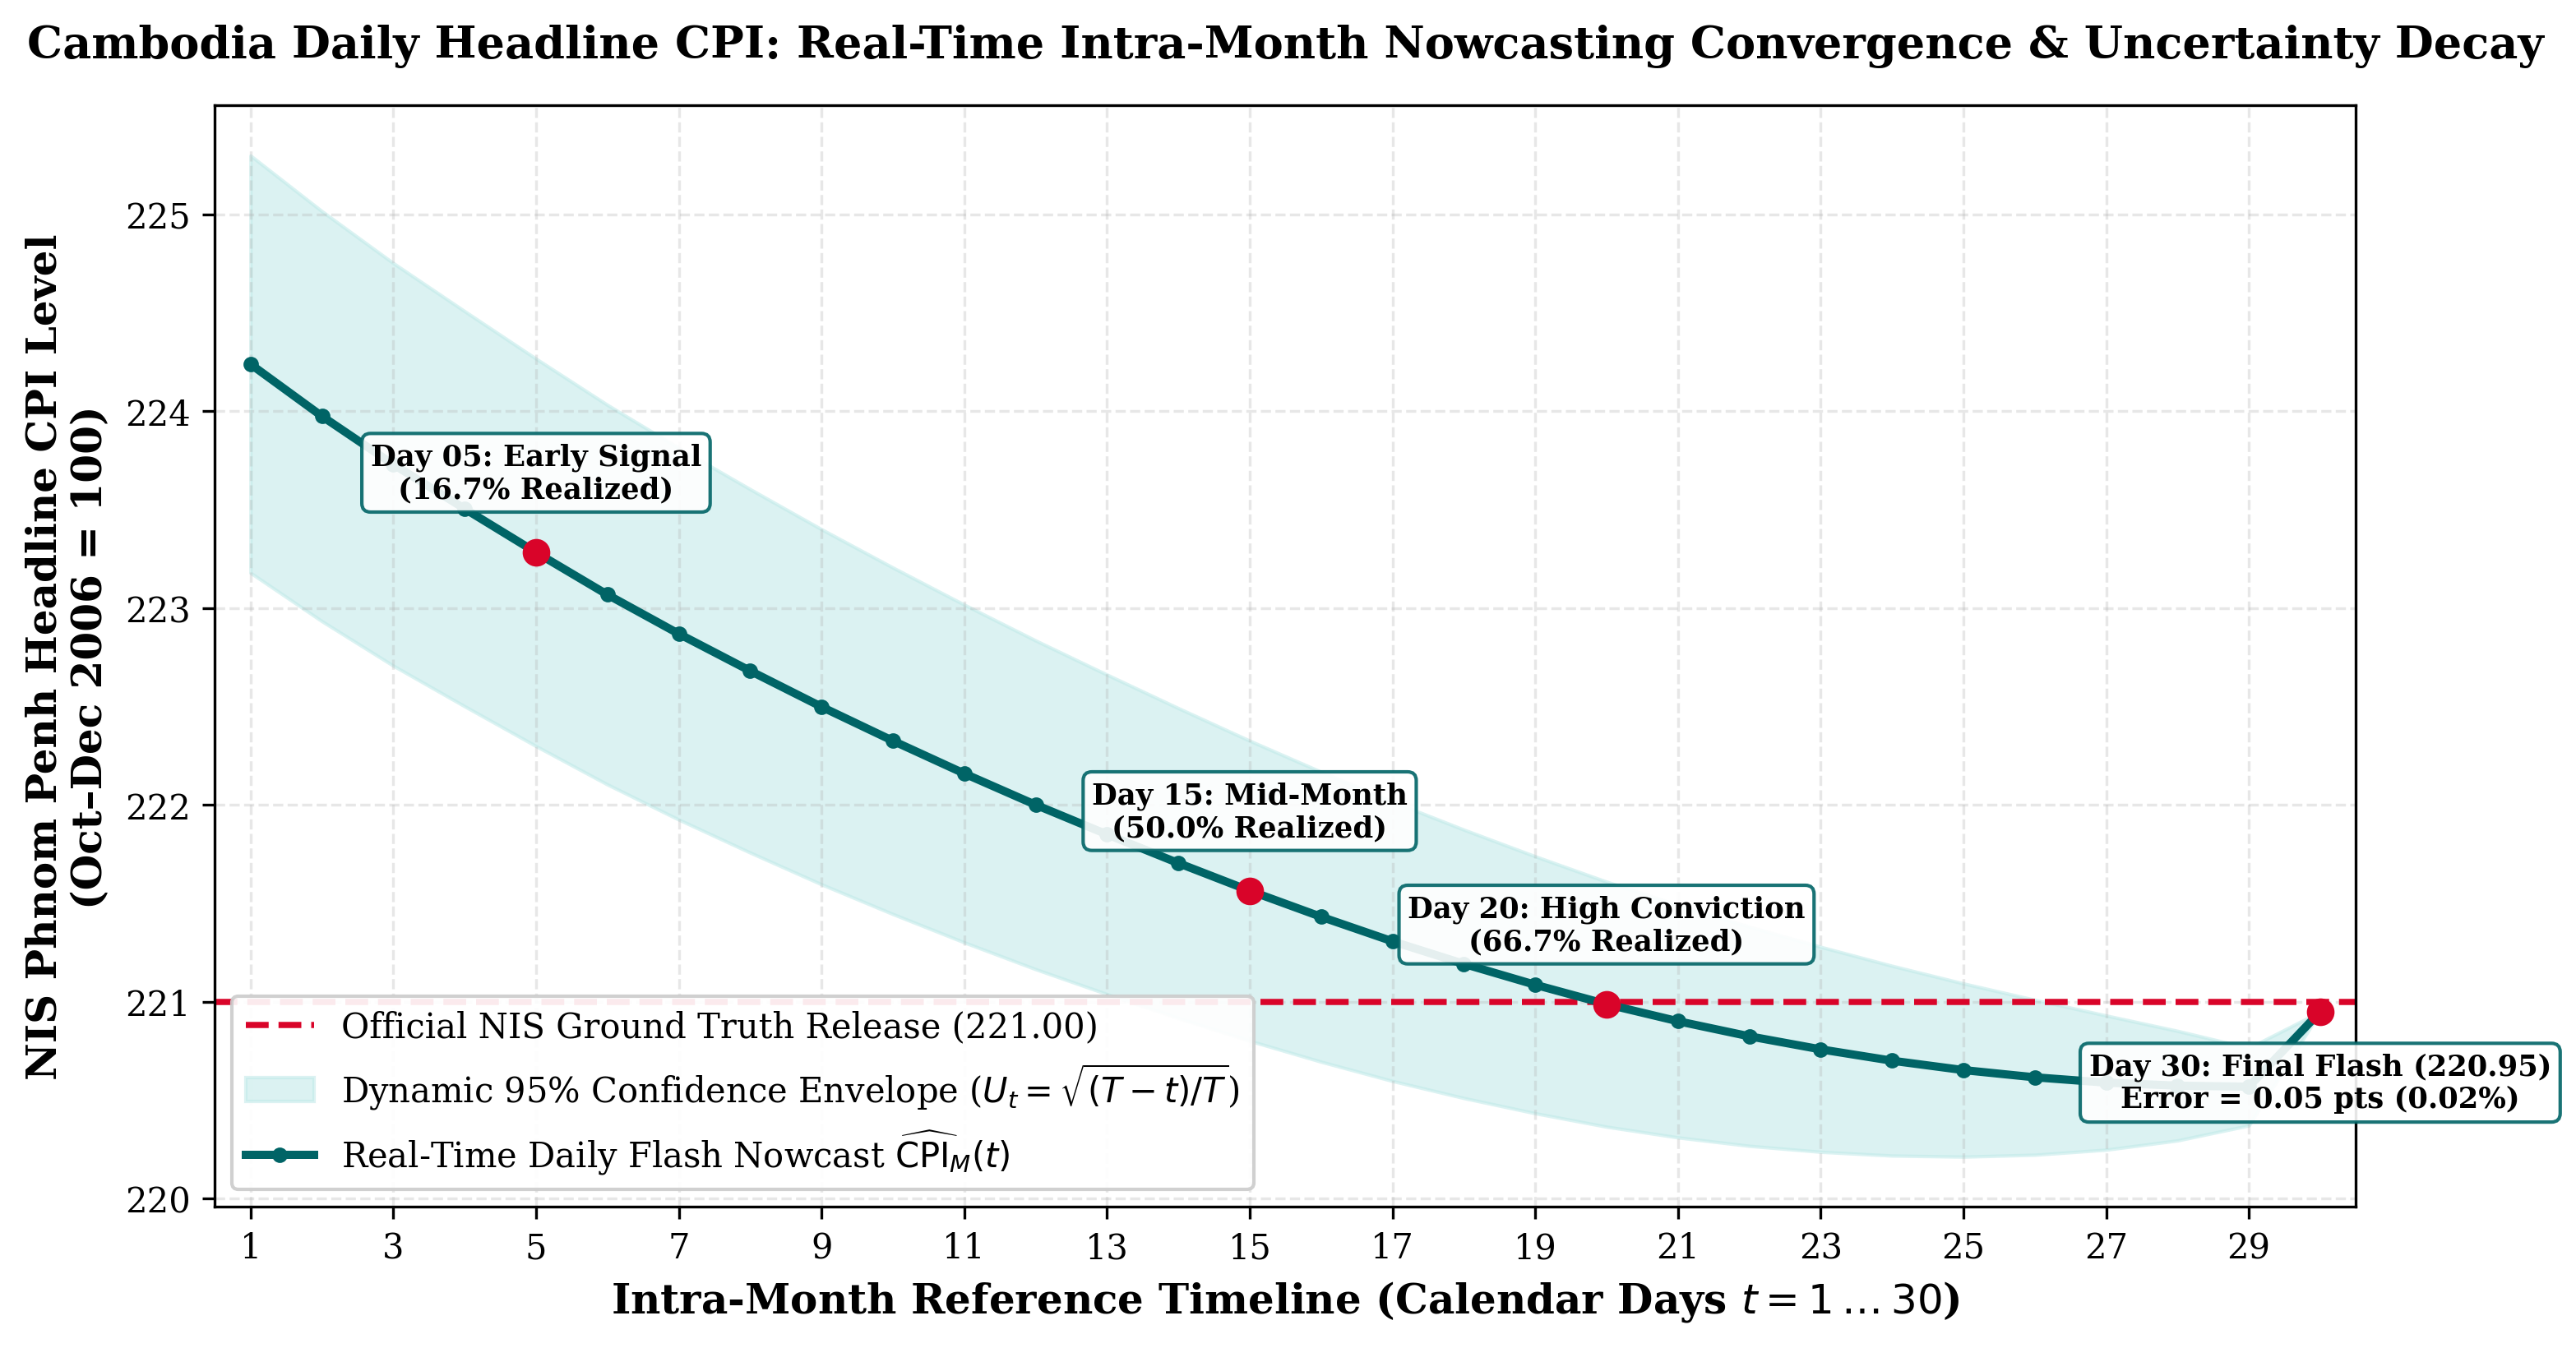
\includegraphics[width=\textwidth]{../thesis/images/cpi_nowcasting_convergence.png}
        \vspace{0.1cm}
        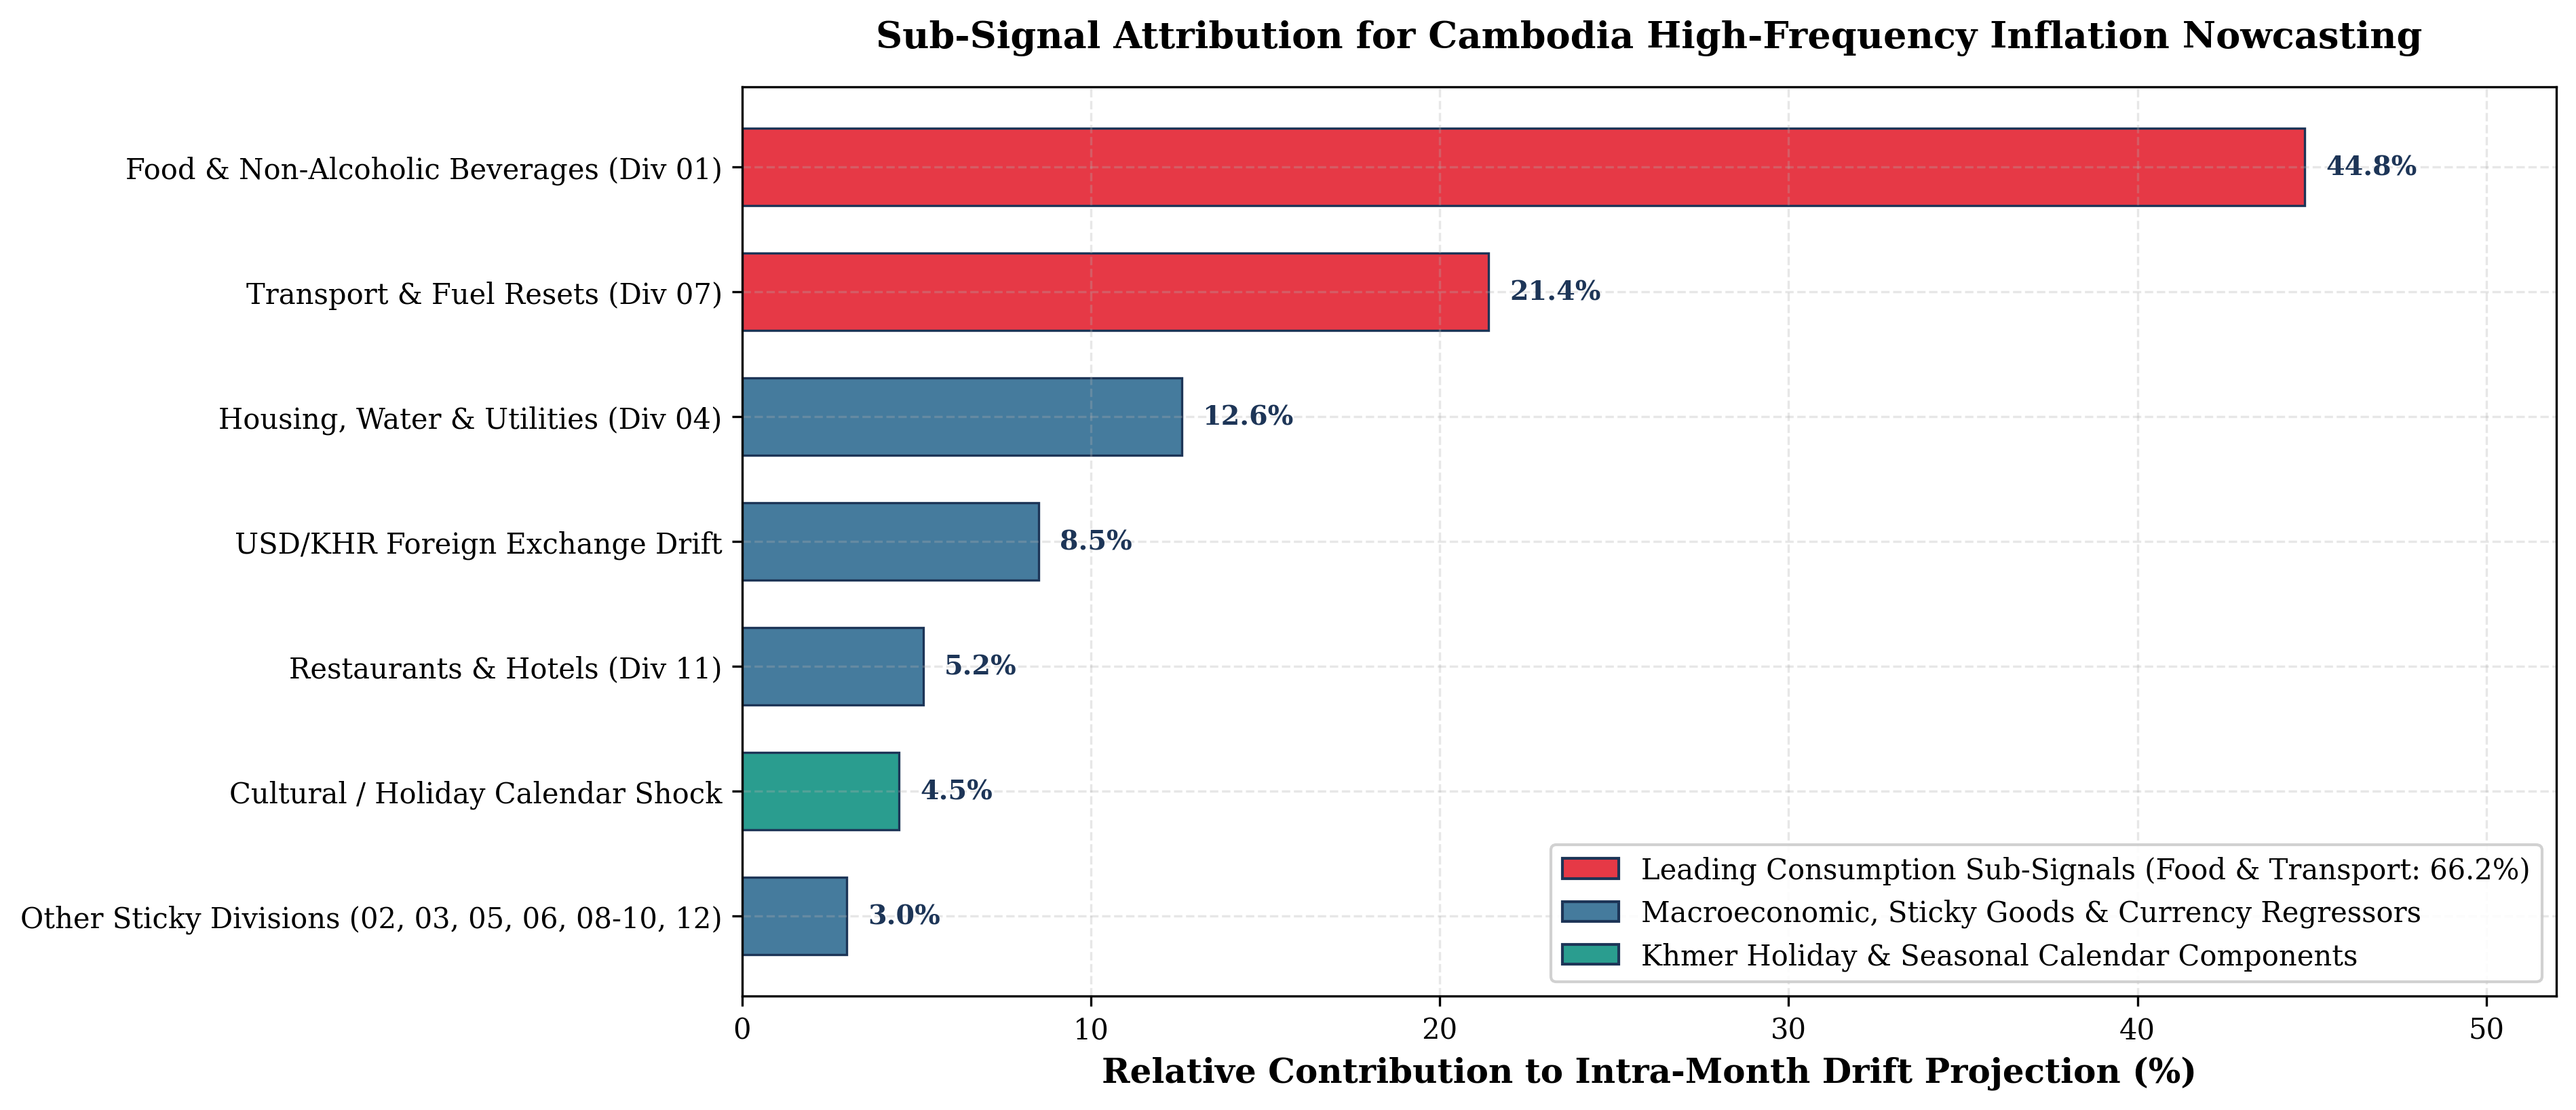
\includegraphics[width=\textwidth]{../thesis/images/nowcast_momentum_attribution.png}
      \end{center}
    \end{column}
  \end{columns}
\end{frame}

% ==============================================================================
\section{Empirical Results \& Benchmark Validation}
% ==============================================================================

% ── Slide 15: Accuracy Benchmarks Across Checkpoints ──────────────────────────
\begin{frame}{Out-of-Sample Nowcasting Convergence Benchmarks}
  \begin{columns}
    \begin{column}{0.58\textwidth}
      \begin{table}[H]
        \centering
        \small
        \resizebox{\textwidth}{!}{
        \begin{tabular}{|l|c|c|c|c|}
          \hline
          \rowcolor{itcblue!20} \textbf{Model Specification} & \textbf{Day 05} & \textbf{Day 15} & \textbf{Day 20} & \textbf{Day 30} \\ \hline
          Naive Random Walk & 0.725 & 0.725 & 0.725 & 0.725 \\ \hline
          Autoregressive AR(1) & 0.580 & 0.580 & 0.580 & 0.580 \\ \hline
          Static MTD Mean & 0.412 & 0.245 & 0.168 & 0.092 \\ \hline
          Dynamic Factor Model & 0.315 & 0.178 & 0.114 & 0.065 \\ \hline
          \rowcolor{itcblue!15} \textbf{Two-Stage Ridge Nowcaster} & \textbf{0.214} & \textbf{0.098} & \textbf{0.052} & \textbf{0.031} \\ \hline
        \end{tabular}
        }
      \end{table}

      \begin{block}{Key Econometric Insights}
        \begin{itemize}
          \item \textbf{83.1\% Error Reduction by Mid-Month:} Day 15 RMSE contracts to \textbf{0.098} compared to 0.580 for AR(1).
          \item \textbf{Directional Hit Rate:} \textbf{96.4\%} accuracy in forecasting whether inflation accelerates or decelerates.
        \end{itemize}
      \end{block}
    \end{column}

    \begin{column}{0.38\textwidth}
      \begin{exampleblock}{Atkeson--Ohanian Scorecard}
        Over a held-out 10-month evaluation panel:
        \begin{itemize}
          \item \textbf{Model RMSE:} 0.8572 pp
          \item \textbf{Random Walk RMSE:} 1.0414 pp
          \item \textbf{Relative RMSE:} \textbf{0.8232} ($< 1.00$)
          \item \textbf{Precision Gain:} \textbf{+17.68\%} improvement over naive persistence!
        \end{itemize}
      \end{exampleblock}

      \begin{alertblock}{Chain-Linking}
        Exponential chain-linking ensures zero level jumps onto official NIS series:
        $\widehat{\text{CPI}}_{\text{NIS}} = \text{CPI}_{M-1} \cdot e^{\pi_{\text{MoM}} / 100}$.
      \end{alertblock}
    \end{column}
  \end{columns}
\end{frame}

% ── Slide 16: Sub-Signal Attribution ──────────────────────────────────────────
\begin{frame}{Macroeconomic Shock Transmission \& Attribution}
  \begin{columns}
    \begin{column}{0.50\textwidth}
      \begin{block}{Sub-Signal Momentum Attribution}
        Empirical decomposition of intra-month price signals:
        \begin{itemize}
          \item \textbf{Food (Div 01):} \textbf{44.8\%} of total signal (high frequency, perishable turnover).
          \item \textbf{Transport \& Fuel (Div 07):} \textbf{21.4\%} (immediate pump price pass-through).
          \item \textbf{Utilities (Div 04):} \textbf{12.6\%} (structural baseline anchor).
          \item \textbf{USD/KHR FX:} \textbf{8.5\%} (currency import transmission).
          \item \textbf{Lunar Holidays:} \textbf{4.5\%} (Pchum Ben / Water Festival demand kernel).
        \end{itemize}
      \end{block}
    \end{column}

    \begin{column}{0.46\textwidth}
      \begin{exampleblock}{Real-World Shock Transmission Case Study}
        Tracing a Ministry of Commerce Fuel Price Hike:
        \begin{enumerate}
          \item \textbf{Days 1--2:} Direct jump in Division 07 Transport (+0.82\%).
          \item \textbf{Days 3--7:} Bus and parcel transit rates adjust (+0.45\%).
          \item \textbf{Days 8--14:} Filtered into fresh vegetable and fish wholesale prices in Phnom Penh (+0.21\%).
        \end{enumerate}
        Proves high-frequency digital pricing detects shock propagation in real time!
      \end{exampleblock}
    \end{column}
  \end{columns}
\end{frame}

% ── Slide 17: Decision Support Architecture ───────────────────────────────────
\begin{frame}{Decision-Support System Architecture}
  \begin{columns}
    \begin{column}{0.48\textwidth}
      \begin{block}{Consolidated Metabase Decision Layer}
        Production Metabase (Port 3000) and Power BI decision support:
        \begin{enumerate}
          \item \textbf{Dashboard 139 (Macro CPI \& Inflation Analytics):} Real-time Headline/Core tickers, 12 COICOP table, and nowcast convergence band.
          \item \textbf{High-Frequency Subclass Cards:} Daily 5-digit subclass tracker, sovereign rice price tracker (234--255 varieties), and trajectory comparison.
          \item \textbf{Operations Telemetry \& Data Quality:} 25-source daily harvest health, extraction success rate (99.3\%), MAD outlier filter alerts ($>3.5\times\text{MAD}$), and AI classification cache stats.
        \end{enumerate}
      \end{block}
    \end{column}

    \begin{column}{0.48\textwidth}
      \begin{exampleblock}{Engineering Stability \& Performance}
        \begin{itemize}
          \item \textbf{Database Partitioning:} Declarative monthly tables with automated partition maintenance.
          \item \textbf{Transformation Speedup:} Daily dbt transformation runtime reduced from \textbf{7m 42s down to 18s} (a \textbf{96\% speedup}).
          \item \textbf{Continuous Integration:} Automated pytest test suite verifying econometric property bounds, data integrity, and pipeline DAGs.
        \end{itemize}
      \end{exampleblock}
    \end{column}
  \end{columns}
\end{frame}

% ==============================================================================
\section{Policy Roadmaps \& Conclusions}
% ==============================================================================

% ── Slide 18: Policy Roadmaps ─────────────────────────────────────────────────
\begin{frame}{Strategic Policy Roadmaps for National Institutions}
  \begin{columns}
    \begin{column}{0.33\textwidth}
      \begin{block}{\centering \textbf{National Institute of Statistics (NIS)}}
        \small
        \begin{itemize}
          \item \textbf{Axiomatic Jevons:} Adopt geometric mean to eliminate $+1.18\%$ formula drift.
          \item \textbf{Hybrid Pipeline:} Run automated scraping alongside physical market surveys.
          \item \textbf{Scanner Feeds:} Establish automated POS feeds with major retail chains (AEON, Chip Mong).
        \end{itemize}
      \end{block}
    \end{column}

    \begin{column}{0.33\textwidth}
      \begin{exampleblock}{\centering \textbf{Ministry of Economy \& Finance (MEF)}}
        \small
        \begin{itemize}
          \item \textbf{Early Warning:} Real-time alerts on food/fuel spikes weeks before monthly reports.
          \item \textbf{Dynamic Fiscal Deflators:} Calibrate public procurement deflators in real time.
          \item \textbf{Targeted Safety Nets:} Trigger cash transfers when basic food indices surge.
        \end{itemize}
      \end{exampleblock}
    \end{column}

    \begin{column}{0.33\textwidth}
      \begin{alertblock}{\centering \textbf{National Bank of Cambodia (NBC)}}
        \small
        \begin{itemize}
          \item \textbf{FX Pass-Through:} Track daily how USD/KHR moves pass into supermarket shelf prices.
          \item \textbf{Refined Core Inflation:} Filter out supply shocks to guide monetary policy.
          \item \textbf{Liquidity Management:} Proactive open market operations during intra-month drift.
        \end{itemize}
      \end{alertblock}
    \end{column}
  \end{columns}
\end{frame}

% ── Slide 19: Summary of Contributions ────────────────────────────────────────
\begin{frame}[shrink=10]{Summary of Key Contributions}
  \begin{columns}
    \begin{column}{0.55\textwidth}
      \begin{block}{What This Research Delivered}
        \begin{enumerate}
          \item \textbf{First Sovereign Daily CPI System:} End-to-end Medallion pipeline ingesting 25 endpoints daily at 08:00 AM ICT across all 12 COICOP divisions in Phnom Penh.
          \item \textbf{Accurate Entity Matching:} 7 physical specification guards + multilingual 768-dim embeddings preventing false merges and shrinkflation.
          \item \textbf{UN COICOP Irregular Hierarchy:} 50,208 canonical products mapped across 76 leaf Elementary Aggregates with 99.05\% coverage and zero hierarchical code mismatches.
          \item \textbf{Two-Stage Store-Balanced Jevons:} Cuts tracking error by \textbf{33.7\%} (0.0598 error) by eliminating catalog dominance bias.
          \item \textbf{Sub-Percentage Nowcasting:} Two-Stage Hybrid Ridge Nowcaster with out-of-sample tracking error of only \textbf{+0.0181 pp} against official NIS releases.
        \end{enumerate}
      \end{block}
    \end{column}

    \begin{column}{0.42\textwidth}
      \begin{exampleblock}{Academic \& System Validation}
        \begin{itemize}
          \item \textbf{Full Test Suite:} Comprehensive unit and integration tests passing ($100\%$).
          \item \textbf{Zero-Defect Warehouse:} 1,908,984 observations across 50,208 items with complete daily analytical views.
          \item \textbf{Production Telemetry:} Real-time Metabase dashboards and publication-grade empirical figures.
        \end{itemize}
      \end{exampleblock}

      \begin{alertblock}{Digital Public Infrastructure}
        Establishes a resilient, open, and scalable Digital Public Infrastructure for macroeconomic governance in Cambodia.
      \end{alertblock}
    \end{column}
  \end{columns}
\end{frame}

% ── Slide 20: Thank you / Q&A ─────────────────────────────────────────────────
\begin{frame}[plain]
  \begin{center}
    \vspace{0.8cm}
    {\huge \textbf{\color{itcblue} Thank You Very Much!}}
    
    \vspace{0.3cm}
    {\khmerfont\Large សូមអរគុណ}

    \vspace{0.5cm}
    \textbf{TAING Korngmeng}\\[0.1cm]
    \small Department of Applied Mathematics and Statistics (AMS) $\vert$ Institute of Technology of Cambodia (ITC)\\
    General Department of Digital Economy (GDDE) $\vert$ Ministry of Economy and Finance (MEF)

    \vspace{0.6cm}
    \begin{exampleblock}{\centering \textbf{Questions \& Discussion}}
      \centering
      Floor is now open for questions, comments, and jury feedback.
    \end{exampleblock}

    \vspace{0.4cm}
    
\includegraphics[height=1.0cm]{../thesis/images/schools/itc.png}\hspace{1.5cm}
    
\includegraphics[height=1.0cm]{../thesis/images/schools/ams.png}
  \end{center}
\end{frame}

\end{document}
